\documentclass[color,table,oneside,nolot,nolof]{fithesis}
\usepackage[resetfonts]{cmap}
\usepackage[main=czech,english]{babel}
\usepackage[utf8]{inputenc}
\thesissetup{
		university = mu,
		faculty = fi,
		type = bc,
		author = Václav Hodina,
		gender = m,
		advisor = Marek Grác,
		title = {Vizualizace rozdělování disků},
		keywords = {vizualizace, instalace, rozdělení disků, linux, LVM, RAID},
}
\thesislong{abstract}{
	Práce popisuje vývoj modulu do instalátoru Anaconda, který využívají linuxové distribuce vycházející z~Red Hat Enterprise Linuxu.
}
\thesislong{thanks}{
	Zde chci poděkovat Marku Grácovi za vedení mé práce, Marii Staré za korektury.
}
\usepackage{csquotes}
\usepackage[plainpages=false,pdfpagelabels,unicode]{hyperref}
\usepackage{charter,graphicx}
\usepackage[top=1in, bottom=1.25in, left=1.25in, right=1.25in]{geometry}
\usepackage[
	backend=biber,
	style=numeric,
	citestyle=numeric-comp,
	sorting=none,
	sortlocale=auto
	]{biblatex}
\addbibresource{bak_prace.bib}
\usepackage{makeidx}
\makeindex
\usepackage{paralist} 
\usepackage{amsmath} 
\usepackage{amsthm} 
\usepackage{amsfonts} 
\usepackage{url} 
\usepackage{menukeys}
\hyphenation{graph-viz}
\begin{document}
\chapter{Úvod}
	Bakalářská práce zpracovává řešení problémů s~vizualizací rozdělených disků při instalaci systému. Cílem práce je vytvořit pochopitelnou grafickou nápovědu pro administrátory 
	počítačů, zvláště serverů s~mnoha disky. 
	Konkrétněji se jedná o~rozšíření instalátoru Anaconda, které zpracovává informace o~jednotlivých discích, jako je název, velikost a typ disku a~jednotlivé oddíly na disku utvořené. 
	Samozřejmostí je zahrnutí 
	diskových polí typu RAID (Redundant Array of Independent Disks)  a~virtualizovaných disků mezi vizualizovaná data; rozšíření počítá se všemi těmito typy. Data jsou uložena 
	ve vlastních třídách tak, aby programování případné další funcionality 
	nepředstavovalo problém. Program vytváří graf podobný stromové struktuře a~zobrazuje jej uživateli. Graf se během instalace tvoří dvakrát, poprvé
	před rozdělením disků a~podruhé pro kontrolu, zda jsou předložené změny korektní, než se zformátují disky. V~současnosti je k~tomuto účelu využíván pouze textový 
	seznam změn, který je nedostatečný. Člověk dokáže mnohem lépe a~rychleji kontrolovat obrázková data než homogenní text. 

	Práce vznikala nejen na Fakultě informatiky Masarykovy univerzity (FI MUNI), ale i~ve společnosti Red Hat. Tam budou využity její výsledky,
	integrované do instalátoru Anaconda, který je v~současnosti používán v~linuxových distribucích Red Hat Enterprise Linux (RHEL), CentOs a~Fedora.

	Práci jsem si vybral z~několika důvodů.  Možnost podílet se na vývoji svobodného softwaru je pro mě velmi důležitým hlediskem 
	při psaní jakéhokoliv programu. Druhý důvod je možný rozsah uplatnitelnosti výsledků mé práce. Každý systém je třeba nejprve nainstalovat, výsledky
	této práce tedy uvidí velké množství lidí, což je bezpochyby velká motivace pro každého, kdo něco tvoří. Třetím důvodem je výběr programovacího jazyka, který je vyžadován 
	v~zadání. Jedná se o jazyk Python, který považuji za velmi flexibilní, aniž by byly kladeny přílišné nároky na výkon systému. 

	Jak jsem zmínil výše, hlavním cílem práce je naprogramování aplikace, která vytváří graf stromové struktury rozdělených disků. Data přijímá od instalátoru Anaconda, 
	přičemž využívá knihovnu blivet. 
	Vedlejšími cíli je možnost vytvářet grafy ze souborů XML, ne jen z~aplikace, dále integrace do instalátoru s~možností označovat jednotlivé diskové oddíly a~interagovat
	s~nimi. Posledním doplňkovým cílem je funkcionalita umožňující porovnat stav před instalací a~po ní v~případě, že je systém přeinstalováván.

	Z~cílů vychází také struktura práce. Před popisem je přidána přehledová kapitola.
	První kapitola popisuje použité knihovny. První knihovna, blivet\cite{blivet}, poskytuje data a mimo jiné může sloužit i~pro změny 
	nastavení disků (tato funkcionalita je v~mé práci zmíněna jen okrajově). Druhou je knihovna graphviz-python\cite{graphviz-python}, Graphviz je program pro tvorbu grafů. Kromě
	jednoduchého spojování uzlů hranami dokáže uzly automaticky třídit a~logicky rozmisťovat podle různých přednastavených pravidel. Nabízí také různý vzhled uzlů
	a~hran a výsledné grafy dokáže exportovat v~několika formátech. Výsledek mé práce operuje především s~formátem škálovatelné vektorové grafiky (SVG). Graphviz-python je 
	nadstavba Graphvizu pro použití v~jazyce Python.

	Druhá kapitola je o~mém návrhu jednotlivých tříd programu, jejich dokumentaci a~popisu funkcí. Nejdůležitější z tříd jsou ty pro uzly a~hrany. Zmíněny jsou také pomocné třídy 
	pro načítání z~jiných formátů vstupních dat, jako je již zmiňované XML.

	Třetí kapitola obdobně popisuje návrh vzhledu aplikace a~její chování. Zdůvodňuje, proč jsem se rozhodl pro jednotlivé grafické prvky a~barevná odlišení.

	Čtvrtá kapitola obsahuje ukázky práce programu. Demonstruje několik konfigurací, jež mají za úkol program otestovat a~vyzkoušet i~potenciálně problémové situace. Ukázky  
	zahrnují situace jak při práci v~prostředí instalátoru, tak mimo něj.

	Pátá kapitola zmiňuje další možná rozšíření mého programu. 

\chapter{Přehledová kapitola}
\section{Současný stav}

V~současné době je vizualizace rozdělení disků při instalaci systému použita v~minimu případů. Dále v~kapitole rozebírám jednotlivé ukázky programů, které jsem vybral, avšak souhrnně je vidět, 
že instalátory se drží textového seznamu diskových oddílů uspořádaných do stromové struktury. Systémy jsem vybíral tak, aby bylo možné porovnat alespoň nějakou vizuální stránku. Proto jsem vynechal
příklady typu Archlinux či Gentoo, které používají pouze instalaci z~příkazové řádky.  Dále uvádím příklady vizualizace, kterou používají nástroje na práci s~disky, jako je 
například program GParted.

\section{Příklady instalátorů v různých operačních systémech}

\subsection{Debian}

Prvním příkladem je Debian, velmi konzervativní distribuce udržující osvědčené postupy a~programy, snažící se o~maximální stabilitu i~za cenu zastaralosti. 
Tato distribuce má grafický instalátor, spoléhá ovšem na zkušenosti a~znalosti uživatele. Během instalace se k~žádnému schématu nedostaneme. Jak je vidět na obrázku č. 1, jediný způsob předání 
informace o~plánovaném stavu disku je textový strom diskových oddílů obohacený o~možnost výběru a~ovládání myší.

\begin{figure}[hb]
	\caption{Distribuce Debian}
	\centering
	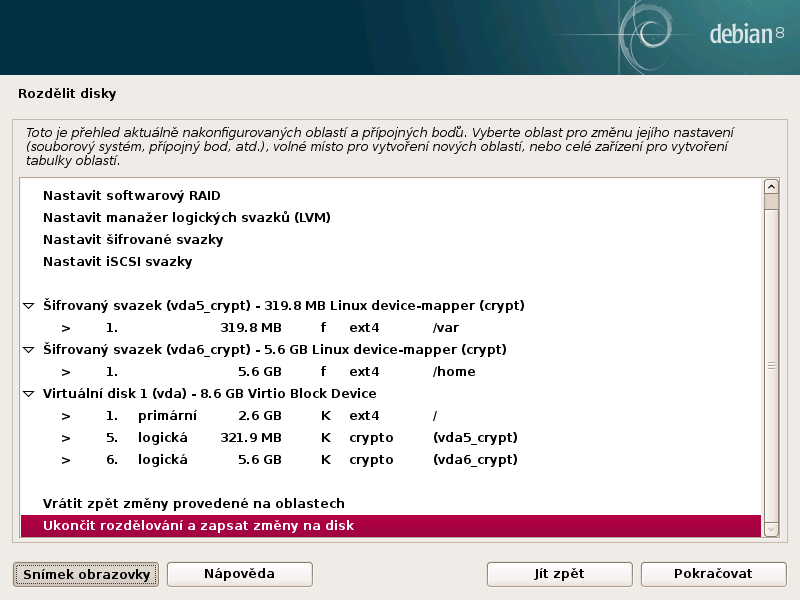
\includegraphics[width=.6\columnwidth]{pics/debian1.png}
\end{figure}

\subsection{Ubuntu}

Ubuntu Linux vychází z~výše zmíněné distribuce Debian, instalátor však používá svůj vlastní. Je také jediným zástupcem linuxové distribuce, která využívá  schéma 
pro znázornění stavu rozděleného disku. Dříve využívané schéma programu GParted, které detailně rozebírám dále, bylo nahrazeno jednoduchou linkou v~horní oblasti okna instalátoru. Na této lince 
jsou barevně znázorněny diskové 
oddíly vytvořené uživatelem. Stejné barvy jsou poté použity u~každého ze záznamů v~seznamu oddílů, jak je možné vidět na obrázku č. 2. Tento jednoduchý diagram umožňuje rychlý odhad poměrů různých 
částí, které budou vytvořeny.

\begin{figure}[hb]
	\label{fig:ubuntu}
	\caption{Distribuce Ubuntu}
	\centering
	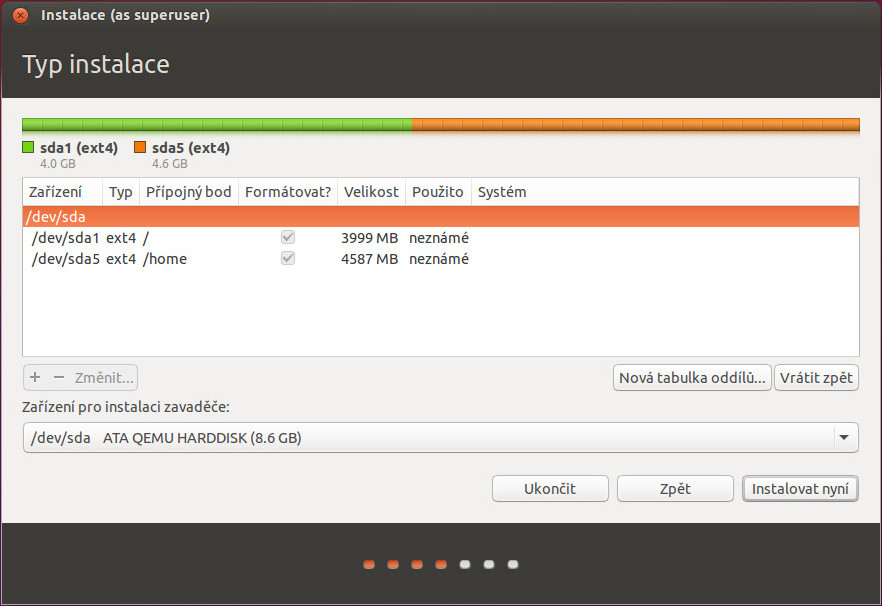
\includegraphics[width=.6\columnwidth]{pics/ubuntu1.jpg}
\end{figure}

\subsection{CentOS}

Jako příklad systémů, které využívají instalátor Anaconda, jsem vybral systém CentOS. Tato zkratka znamená Community ENterprise Operating System. Na svých stránkách uvádějí \uv{The CentOS Linux
distribution is a~stable, predictable, manageable and reproducible platform derived from the sources of Red Hat Enterprise Linux (RHEL).}~\cite{CentOS}. Jedná se v~podstatě o~systém Red Hat Enterprise 
Linux, ovšem bez podpory a~oprav od společnosti Red Hat. V~současné době instalátor Anaconda používá také pouze textovou reprezentaci rozdělení disku. Rozdíl oproti ostatním distribucím tvoří 
seznam změn, který je zobrazen před finálním potvrzením a~započetím formátování. Na obrázku č. 3 můžeme vidět příklad tohoto seznamu. Situaci zpřehledňuje ale pouze pro malý počet změn, seznam s~mnoha 
záznamy o~změnách je nepřehledný. Zlepšením uživatelské přívětivosti při finální kontrole před instalací se zabývá tato práce.

\begin{figure}[h]
	\label{fig:centos2}
	\caption{Distribuce CentOS příklad souhrné tabulky}
	\centering
	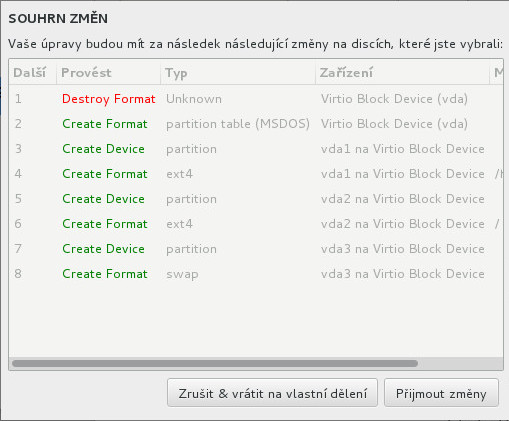
\includegraphics[width=.6\columnwidth]{pics/centos3.jpg}
\end{figure}

\subsection{Windows 10}

Pro srovnání uvádím i~příklad nejrozšířenějšího systému, MS Windows. Vybral jsem v~současnosti nejnovější verzi, Windows 10. Překvapivě ani zde nejsou využity vizuální pomůcky.
Tvůrci instalátoru spoléhají na automatickou instalaci a~rozdělení disku s~tím, že pokročilou verzi s~manuálním nastavováním zvolí uživatel, který se zorientuje během instalace i~bez grafické nápovědy. 
Předchozí verze využívají stejný systém jako má distribuce Ubuntu, tj. obdélník znázorňující disk, v~němž jsou barevně vyznačeny diskové oddíly.

\begin{figure}[h!]
	\label{fig:win}
	\caption{Systém Windows}
	\centering
	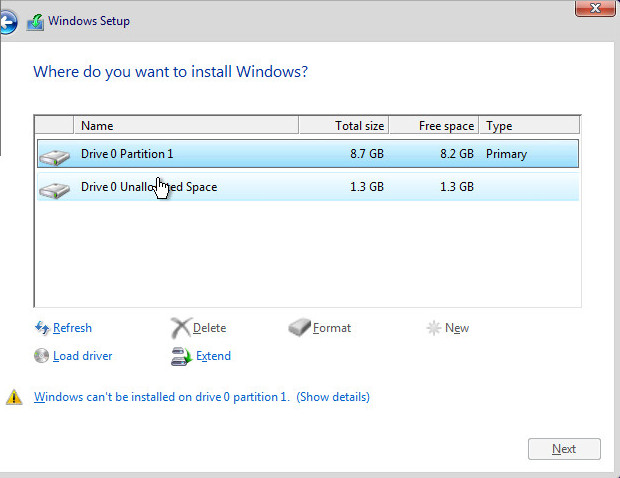
\includegraphics[width=.6\columnwidth]{pics/win1.jpg}
\end{figure}

\section{Programy sloužící pro manipulaci s~disky}

\subsection{GParted}

Program GParted je zástupcem programů, které je možné spouštět i~mimo fázi instalace systému. Dříve byl součástí instálátoru systému Ubuntu, ale je možné jej spouštět i~samostatně, například 
 zvětšovat úložnou kapacitu virtuálních disků či disků, jejichž souborový systém umožňuje pozdější modifikaci. Opět je využito dříve zmíněné schéma obdélníku. Každý disk je reprezentovaný 
 obdélníkem a~další informace jsou zobrazovány barevnými rámci uvnitř těchto obdélníků. Narozdíl od ostatních zmíněných programů obsahuje GParted i~grafické aplikace pro manipulaci s~disky 
 a~tím dosahuje efektu WYSIWYG editoru (What You See Is What You Get, editor, který přímo ukazuje aktuální změny). Příkladem je aplikace pro zvětšení diskového oddílu, kterou vidíme na obrázku č.~5.

 \begin{figure}[h!]
	 \label{fig:gparted}
	 \caption{Ukázka widgetu pro program GParted~\cite{GParted}}
	 \centering
	 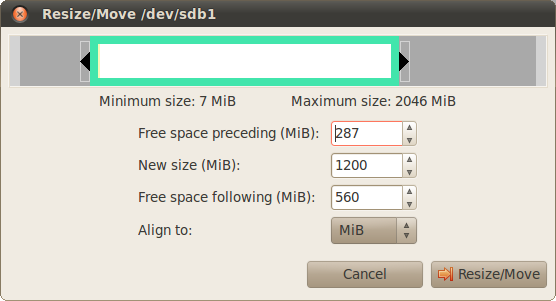
\includegraphics[width=.6\columnwidth]{pics/gparted-5-big.png}\\
 \end{figure}

 \subsection{Blivet-gui}

 Druhým příkladem je program na manipulaci s~disky, který je součástí instalátoru Anaconda, využívá knihovnu nazvanou blivet. Knihovna blivet je základem pro všechny systémy vycházející ze systému RHEL. Autoři 
 se zprvu rozhodli použít známé schéma, avšak brzy narazili na problém s~větším počtem disků včetně virtuálních. Na obrázku č.~6 vidíme, že současné řešení je nedostatečné, jednotlivé úrovně barevných rámců 
 jsou znázorněny samostatnými uzly grafu s~hranami vyznačujícími vztahy mezi nimi. Mnoho těchto rámců uživatele spíše zmate a~použití grafu by situaci zpřehlednilo.

 \begin{figure}[h!]
	 \label{fig:blivet}
	 \caption{Ukázka programu blivet-gui~\cite{blivet-gui}}
	 \centering
	 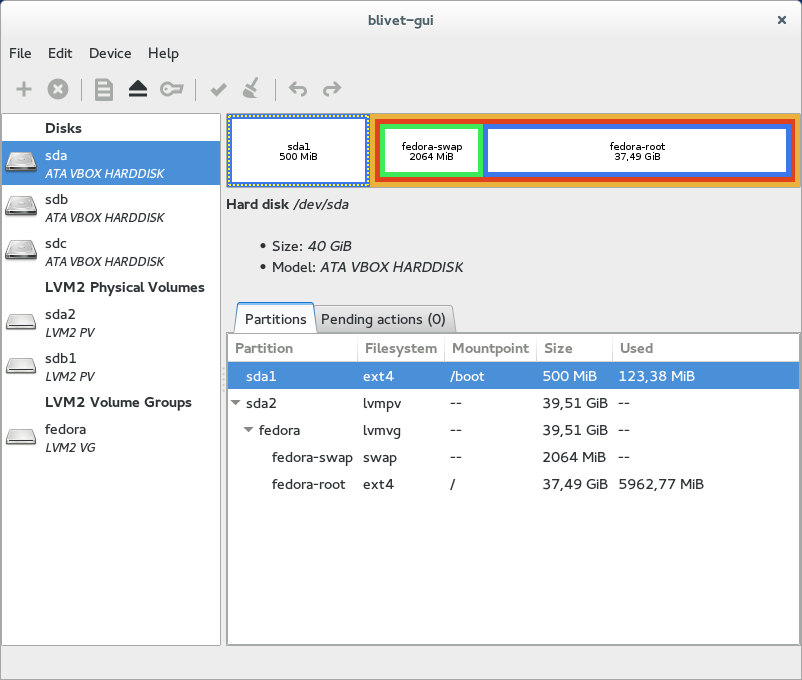
\includegraphics[width=.6\columnwidth]{pics/blivet-gui-1.png}\\
 \end{figure}

\chapter{Použité knihovny}
\section{Knihovna Blivet}
	První a nejdůležitější knihovouk která je v mé práci využívána je knihovna blivet. Jde o projekt a bakalářsknou práci Bc. Vojtěcha Trefného. Projekt vznikl, stejně jako moje
	práce ve firmě Red Hat a slouží k rozšíření již zmiňovaného instalátoru Anaconda. Použití této knihovny je součástí zadání a proto nebudu diskutovat její výhody a nevýhody
	oproti ostatním knihovnám. 

	Blivet však není knihovnou která by jen četla informace o pevných discích. Mezi její funkce patří i konfigurace různých datových úložišť. Nemusí se ani jednat jen o pevné disky.
	Ovládá i mnohé další technologie se kterými se lze v dnešní době setkat. Příkladem jsou to vícenásobné pole nezávislých disků (RAID), technologie logických svazků disku (LVM) či 
	ovládání zašifrovaných modulů pomocí technologie LUKS. Všechny 3 příklady proberu níže.

	Dále obsahuje též nástroje pro práci se souborovými systémy diskových oddílů od starších a již používaných jako jsou žurnálovací souborové systémy ext2 až ex4 či ReiserFS po novější
	jakými jsou btrfs nebo ZFS. Též se stará o bootovací oddíly čili master boot record (MBR) a GUID partition table (GPT). Stručně řečeno stará se o všechny součásti procesu instalace
	nového systému na počítač.

\subsection{RAID}
	Vícenásobná pole nezávislých disků jsou velmi elegantní ochranou před selháním disků. Existůjí různé způsoby jak pole realizovat ale základní princip zůstává vždy stejný. Jde v~něm
	o~několik disků, které nakonec vystupují jako jeden disk. Podle použítí typu vícenásobného diskového pole může mít tento disk kapacitu rovnou součtu disků jej tvořících, anebo také
	jen kapacitu jednoho disku, přičemž data jsou zrcadlena na ostatní disky. Cílem tohoto nastavení je ochrana před selháním hardware a ztrátou dat. 
	
	Blivet obsahuje nástroje pro práci s svobodnou technologií mdadm která slouží k nastavení softwarového RAID pole. Při využití hardwarových technologií, zvláště pak nesvobodných
	je možné k tomuto RAIDu přistupovat jako k obyčejnému disku, čehož i nesvobodné RAIDy často využívájí a svých mnoho disků schovávají za jednotným rozhraním, které se tváří jako jeden
	disk. 

	Program mdadm je ale softwarový RAID a proto má počítač celou dobu přehled nejen o finálním zabezpečeném disku proti selhání ale i o všech dílčích discích které ho tvoří. Výhodou je
	možnost monitoringu redundantních disků nástroji které jsou součástí systému, bez nutnosti využívání aplikací třetích stran u kterých je možnost nekompatibility případně dalších 
	komplikací.
	Mezi nevýhody se řadí větší nepřehlednost při práci se všemi disky počítače, kdy změna jednoho disky vyvolává řetězovou reakci dalších změn. Právě proto je třeba data uceleně třídit
	a pokud možno i přehledně vizualizovat.

\subsection{LVM}
  LVM neboli logical volume management je metoda, kterou je možno spravovat diskové oddíly. Poskytuje větší flexibilitu volného místa než klasické diskové oddíly. Pracuje se třemi
	úrovněmi
	diskových zařízení. Prvnímy jsou fyzické svazky neboli physical volumes (PV). Fyzický svazek je tvořen buď samotným diskem, včetně například RAID disku, nebo diskovým oddílem. 
	Fyzické
	svazky nenabízí o mnoho více funkcionality než je označení a příparava svazku pro další práci. Příprava spočívá v rozdělení fyzického svazku na fyzické extenty (physical extents, PE).

	Další úrovní jsou skupiny svazků (volume groups, VG), sdružující jak jeden nebo více fyzických svazků tak logických svazků. Skupiny svazků disponují úložným prostorem svých PV, 
	který rozdělují mezi logické svazky. Výhodou existence VG je možnost libovolně přidávat svazky a to i za plného chodu systému. Za chodu systému lze místo i ubírat ale samozřejmě
	pouze dosud neobsazenou část. 

	Třetí úrovní jsou již zmíněné logické svazky které jsou dostupné pro uživatele k ukládání jeho dat. Z tohoto pohledu se chovají se stejně jako obyčejné diskové oddíly. Jak již ale
	bylo zmíněno výhodou oproti obyčejným diskovým oddílům je flexibilita dostupného místa. Na logických svazcích je již možné vytvářet souborové systémy a dále s nimi pracovat.

	Kromě úprav velikosti za chodu je také možné přesouvat data mezi jednotlivými skupinami svazků. LVM také umí vytvářet snímky, tj. zachycovat stav dat v čase. Využítí nachází tato 
	vlastnost
	při vytváření záloh a jako záchytný bod ke kterému je možné se vrátit. Nevýhodou logical volume managementu je skutečnost, že data na fyzických svazcích mohou být fragmentována a tak
	dochází ke snížení výkonu. Také je třeba mít na zřeteli fakt, že pokud zmenšujeme logický svazek musí tuto funkci obsahovat i souborový systém který se na něm nachází.

\subsection{LUKS}
	Linux Unified Key Setup (unifikované nastavení klíčů na linuxu) zkráceně LUKS je specifikace šifrování disků původně vytvořená pro systém Linux. Existují i implementace na jiné 
	systémy
	těmi se zde ale zabývat nebudu. Slovy autora LUKS vznikl, aby usnadnil proces nastavování šifrovaných dat: "It has initially been developed to remedy the unpleasantness a user 
	experienced that arise from deriving the encryption setup from changing user space, and forgotten command line arguments. The result of this changes are an unaccessible encryption
	storage."\cite{on-disk-format} V současné době se používá společně s programem dm-crypt, sloužícím jako prostředek k šifrování.

	Při využití v blivetu lze šifrovat disky, diskové oddíly, logické svazky ale též i fyzické svazky. Tj. celé nastavení LVM může být šifrováno jedním klíčem, aktuálně se takto 
	standardně šifruje LVM ve Fedora linuxu pokud uživatel nastaví automatické rozdělení disku s šifrováním. Nemusí se jednat jen o pevné disky ale též o odstranitelná média jako
	CD-ROM nebo USB paměti. Též lze šifrovat odkládací prostor paměti (swap).

\subsection{Formáty souborového systému}
  Jak již bylo zmíněno blivet umí pracovat i s souborovými systémy. Struktura je následující. Výchozí je seznam zařízení reprezentující jednotlivé disky, jejich oddíly a případně
	speciální technologie jako RAID, LVM či šifrování LUKS. Každé zařízení má ale možnost mít i formát, čímž se myslí formát souborového systému. Podporována je většina známých 
	souborových
	systémů které jsou používány dlouhou dobu. Patří mezi ně souborový systém ext, ReiserFS, XFS. Taktéž existuje podpora pro Btrfs (B-tree FS), experimentální souborový systém 
	vyvíjený společností Oracle. Přestože zatím u btrfs neexistuje stabilní verze je mezi distribucemi podporován, neboť nabízí řešení některých problémů současných filesystémů.

\section{Knihovna Graphviz}
	Graphviz je program sloužící k vizualizaci dat formou grafů, ve smyslu orientovaných či neorientovaných. Pomocí něj je možné generovat grafy sloužící k znázornění počítačové sítě nebo
	vztahů mezi určitými objekty. Nelze vytvářet grafy průběhů funkcí či grafy znázorňující vztahy mezi číselnými hodnotami. Jinými slovy graphviz generuje grafy které známe z teorie grafů,
	ale není schopen generovat grafy známé například z ekonomie.

	Program je z velké části napsán v jazyce C ale ve všech v současnosti používaných jazycích pro něj existují obalovací (wrapper) knihovny. Z těchto knihoven se budeme soustředit hlavně na
	knihovnu pro Python 3 která je používána v mé práci. Pokud bychom graphviz spouštěli jako program a pracovali s ním přímo například z příkazové řádky, využívali bychom jeho vlastní jazyk
	na definici grafů nazvaný DOT. Tento jazyk je definovaný následovně:

	"The following is an abstract grammar defining the DOT language. Terminals are shown in bold font and nonterminals in italics. Literal characters are given in single quotes. Parentheses
	( and ) indicate grouping when needed. Square brackets [ and ] enclose optional items. Vertical bars | separate alternatives.
	\begin{quotation}
	graph			:		[ \textbf{strict} ] (\textbf{graph} | \textbf{digraph}) [ ID ] \textbf{\'\{\'} stmt_list \textbf{\'\}\'}
	stmt_list :		[ stmt [ \textbf{';'} ] stmt_list ]
	stmt			:		node_stmt
	|							edge_stmt
	|							attr_stmt
	|							ID '=' ID
	|							subgraph
	attr_stmt	:	(\textbf{graph} | \textbf{node} | \textbf{edge}) attr_list
	attr_list	:	'[' [ a_list ] ']' [ attr_list ]
	a_list  	:	ID '=' ID [ (';' | ',') ] [ a_list ]
	edge_stmt	:	(node_id | subgraph) edgeRHS [ attr_list ]
	edgeRHS		:	edgeop (node_id | subgraph) [ edgeRHS ]
	node_stmt	:	node_id [ attr_list ]
	node_id		:	ID [ port ]
	port			:	':' ID [ ':' compass_pt ]
	|						':' compass_pt
	subgraph	:	[ \textbf{subgraph} [ ID ] ] \textbf{'\{'} stmt_list \textbf{'\}'}
	compass_pt:	(\textbf{n}| \textbf{ne} | \textbf{e} | \textbf{se} | \textbf{s} | \textbf{sw} | \textbf{w}  | \textbf{nw} | \textbf{c} | \textbf{_})"
	\end{quotation}

	Vidíme že hlavnímy elementy při vytváření grafu jsou graph (graf), uzel (node) a hrana (edge). Základní grafy lze tvořit jen s pomocí těchto tří klíčových slov. Nyní je rozeberu detailněji.

\subsection{Graf}
	Klíčové slovo graph uvádí jakýkoliv graf který bude vytvořen. Včetně prvního kořenového grafu. Každý zápis v jazyce DOT tedy musí začínat slovem graph nebo digraph s výjimkou užití slova
	strict. Pokud jej použijeme zamezíme vzniku vícenásobných hran, neboli mezi každým počátečním a koncovým uzlem bude maximálně jedna hrana. 

	Rozdíly mezi slovy graph a digraph jsou zřejmé. Graph označuje graf neorientovaný ve kterém jsou hrany bez šipek na koncích. Slovo digraph je zkrácené spojení directed graph (orientovaný
	graf) a vyjadřuje tedy graf orientovaný ve kterém na koncích hran jsou šipky. Při vizualizaci rozdělení diskového prostoru jsem se rozhodl použít právě orientované grafu neboť považuji za 
	důležité poskytnout uživateli co nejvíce vodítek ke znázornění vztahu rodič -> potomek a orientované hrany jsou ideálním případem pro tuto pomoc. 

	Speciálním případem grafu je i podgraf (subgraph). Grafy mohou být vkládány do sebe. S pomocí podgrafů lze snížit velikost zdrojového kódu v jazyce DOT. Příkladem budiž situace kdy zápisem
	hrany vedoucí od uzlu k podgrafu ( A -- \{B C\}) vytvoříme stejný efekt jako při zápisu každé jednotlivé dvojice mezi uzlem A a uzly B a C (A -- B, A -- C). Dále je možné podgrafy využít
	pro specifikaci odlišných atributů uzlů či hran. V podgrafu lze jednoduše nastavit jiné atributy než ve zbytku grafu.

	Poslední situací pro využití podgrafu je situace kdy chceme uzly shlukovat. V tomto případě je nutné přidat klíčové slovo cluster k názvu podgrafu a určité grafovací stroje tyto uzly 
	napozicují k sobě do skupiny.

\subsection{Uzly}
	Uzly jsou základem každého grafu. V graphvizu jsou definovány svým jménem. Základní graf s jedním uzlem definujeme v jazyce DOT jednoduše a to pomocí: graf { A }. Tento zápis vytvoří
	graf s jedním uzlem uprostřed v jehož středu bude napsán název uzlu, v našem případě "A". Uzly mají mnoho různých atributů od svého jména po url odkazy a atributy HTML formátování. 
	Nejdůležitějšímy ale jsou ty které jsou definovány v základním nastavení. Jsou to tvar uzlu (shape), barva výplně (fillcolor) a jméno (name) nebo nálepka (label). 
	
	Standardně je tvar nastaven na elipsu a barva
	na bílou. Jméno se bere podle identifikátory při vytváření uzlu. Nálepka je rozšířením jména. Pokud je definována jméno nahrazuje a její obsah je vepsán dovnitř uzlu. Od jména se liší právě
	tím že její obsah lze libovolně upravovat, avšak do ní zle ukládat pouze text, jakékoliv speciální formátování nebude zohledněno. Pro vkládání obrázků složí atribut image a pro vkládání
	odkazů atribut url.

	Právě třemi základnímy atributy jsem se rozhodl rozlišovat jednotlivé typy zařízení se kterými pracuje blivet. S pomocí tvaru uzlu odlišuji technologie zařízení. Čím je technologie
	abstraktnější tím zaoblenější tvar má. Pevné disky a jejich oddíly jsou znázorněny čtverci, LVM čtverci se zaoblenými rohy a disky připojené přes síť či šifrování je znázorněno elipsou.
	Pro toto dělení jsem se rozhold abych zachoval konzistenci celého grafu a naváděl uživatele ke schopnosti rozlišit rozdíly jen s pomocí krátkého shlédnutí tvaru.

	Druhým odlišovacím prvkem je barva. Jak její odstím tak sytost. Některé odstíny jsou rezervovány pro odlišení akcí které budou provedeny při konfiguraci. Zelenou barvou jsou vyznačeny
	nově se objevivší prvky, červenou zaniknuvší prvky a oranžovou prvky u kterých došlo ke změnám. Sytost barvy společně s tvarem jasně definují použitou technologii. Barva pomáhá tam kde
	samotný tvar nestačí. Čili pokud používá jak šifrování tak disk připojený přes internet stejný tvar, tak poté k jejich jednoznačnému odlišení dojde použitím sytější a méně syté barvy.

\subsection{Hrany}
	Hrany nejsou tak komplikovanými elementy jako uzly. Jejich základnímy atributy jsou počáteční a koncový uzel. U neorientovaného grafu nelze rozeznat který uzel je počáteční. Hrany 
	nepoužívají tolik atributů jako uzly avšak například nálepku stále mít mohou. Vzhledem k jejich tvaru je u nich zbytečný atribut výplňové barvy (fillcolor) a používá se jen barva 
	"pera".
	Jak již bylo zmíněno v mé praci jsou všechny grafy orientované a tak záleží na pořadí v jakém jsou uzly předány funkci která tvoří hrany. Nicméně směr je vždy od rodiče k potomkovi
	a nikdy naopak.
	
\subsection{Rozložení}
	Ještě se pozastavím nad různými možnostmi rozložení grafu které knihovna nabízí. Základních je 5, dot, neato, fdp, twopi, circo. Ke každému přiložím obrázek a rozeberu jej 
	podrobněji. U každého příkladu je použit stejný vstupní zápis ale výsledky se velmi liší. Vstupní data vypadají takto:
	\begin{quotation}
	graph\{
		A -- B
		B -- C
		C -- D
		D -- A
		D -- E
		D -- F
		G -- B
		G -- E
	\}
	\end{quotation}

	Prvním rozložením je rozložení dot. Oficiální dokumentace k němu říká:
	"dot - "hierarchical" or layered drawings of directed graphs. This is the default tool to use if edges have directionality."\cite{graphviz_layout} (dot - hierarchické neboli
	vrstvené výkresy orientovaných grafů. Jedná se o standardní nástroj použitý pokud jsou hrany orientované.) Rozhraní dot přehledně udržuje hierarchii mezi rodiči a potomky. Skládá
	své uzly do stromu a proto by mohl být kandidátem na použití v mé práci. Lidé jsou zvyklí vnímat data ohledně úložného prostoru ve formě stromů. Tím pádem jde o intiutivnější
	reprezentaci.

	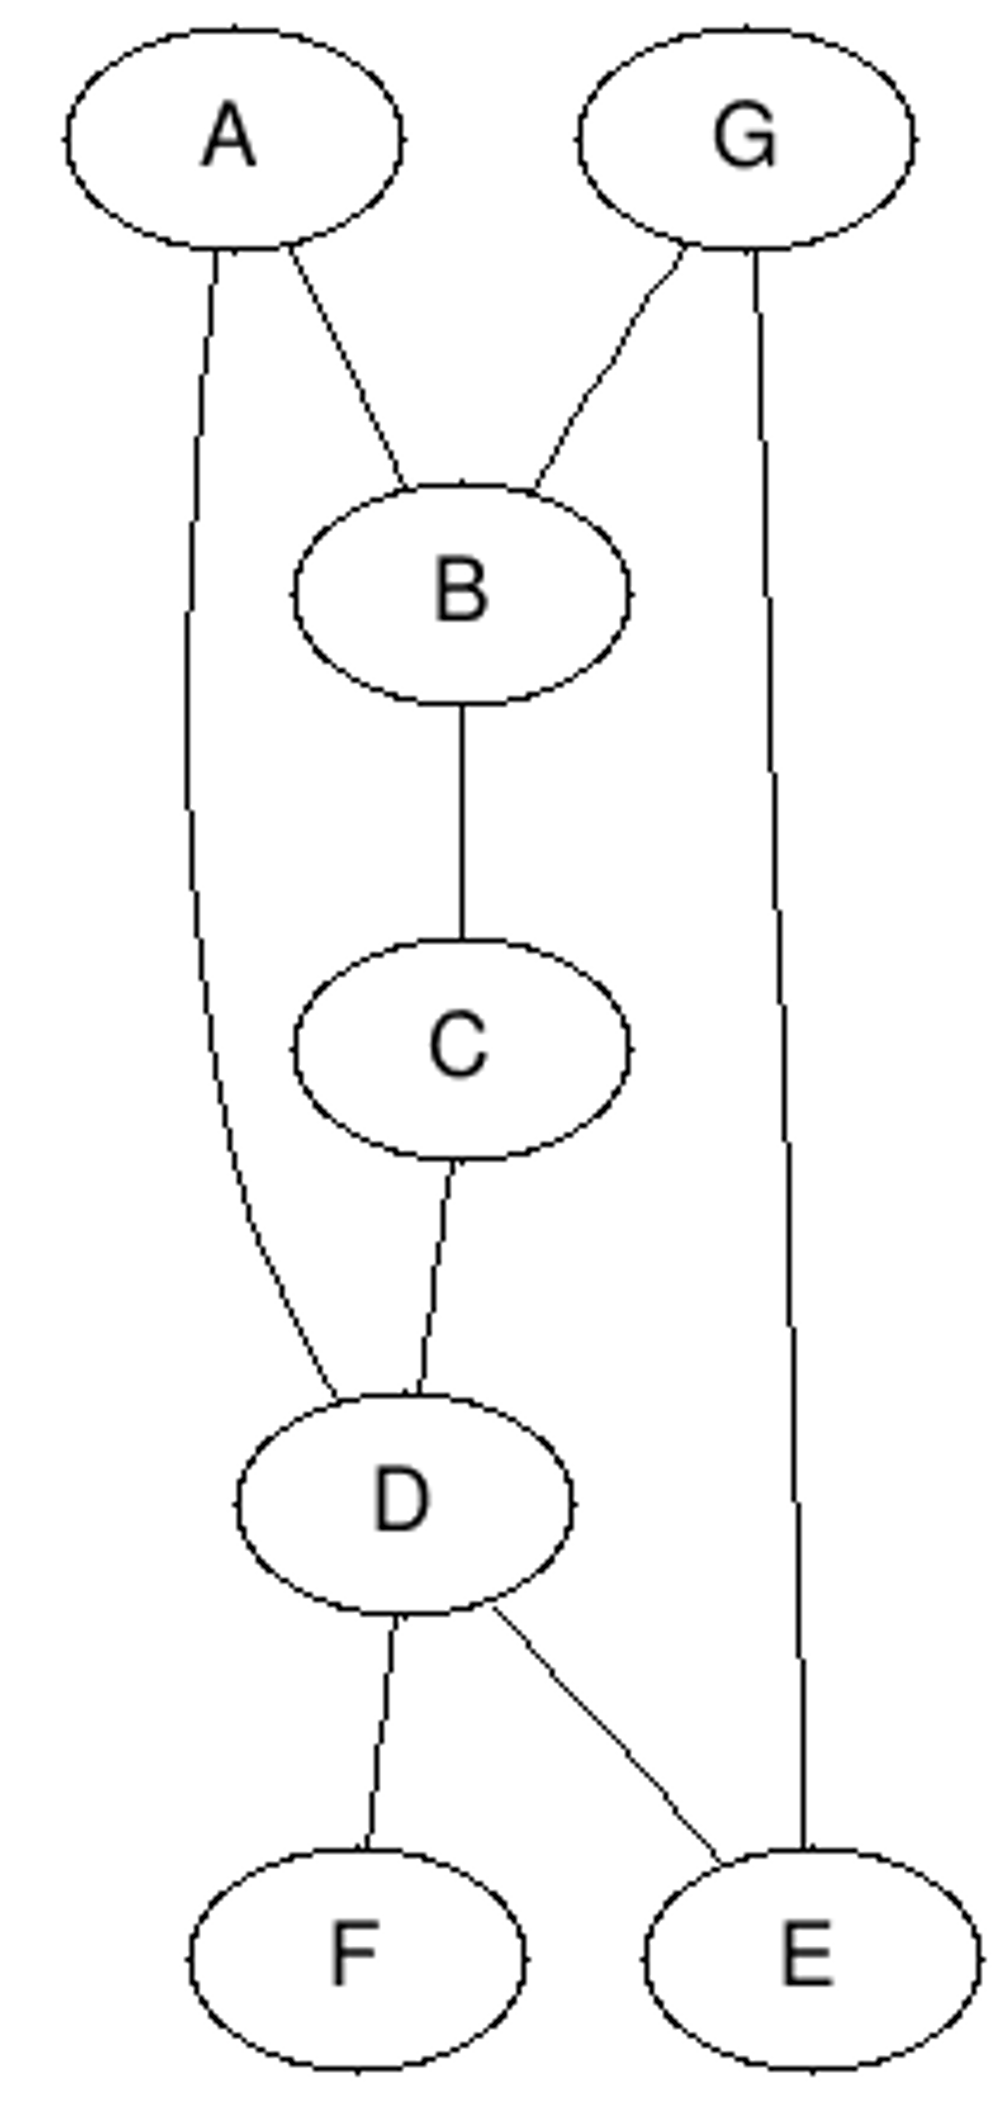
\includegraphics[width=0.6\textwidth]{pictures/dot_example.png} 
	%TODO vysvětli globální energetickou funkci v grafech.
	"neato - \"spring model\" layouts.  This is the default tool to use if the graph is not too large (about 100 nodes) and you don't know anything else about it. Neato attempts to
	minimize a global energy function, which is equivalent to statistical multi-dimensional scaling."\cite{graphviz_layout}(neato - grafy s "pérovacím modelem". Toto je základní nástroj
	používaný pokud je graf malý (má méně než 100 uzlů) a nejsou o něm známy žádné další informace. Neato se pokouší minimalizovat globální energetickou funkci, ekvivalentní
	statistickému multidimenznímu škálování.) Jinými slovy algoritmus neato se snaží vytvořit celý graf co nejmenší bez ohledu na ostatní faktory. Grafy nejsou hierarchické ani 
	strukturované. Cílem je co nejmenší zabraná plocha a zároveň nepřekrývání hran a uzlů. Kvůli chaotičnosti a nestrukturalizovanosti se nejedná o grafový algoritmus který bych mohl
	použít. Ostatně neato je přizpůsobeno na neorinetované grafy.
	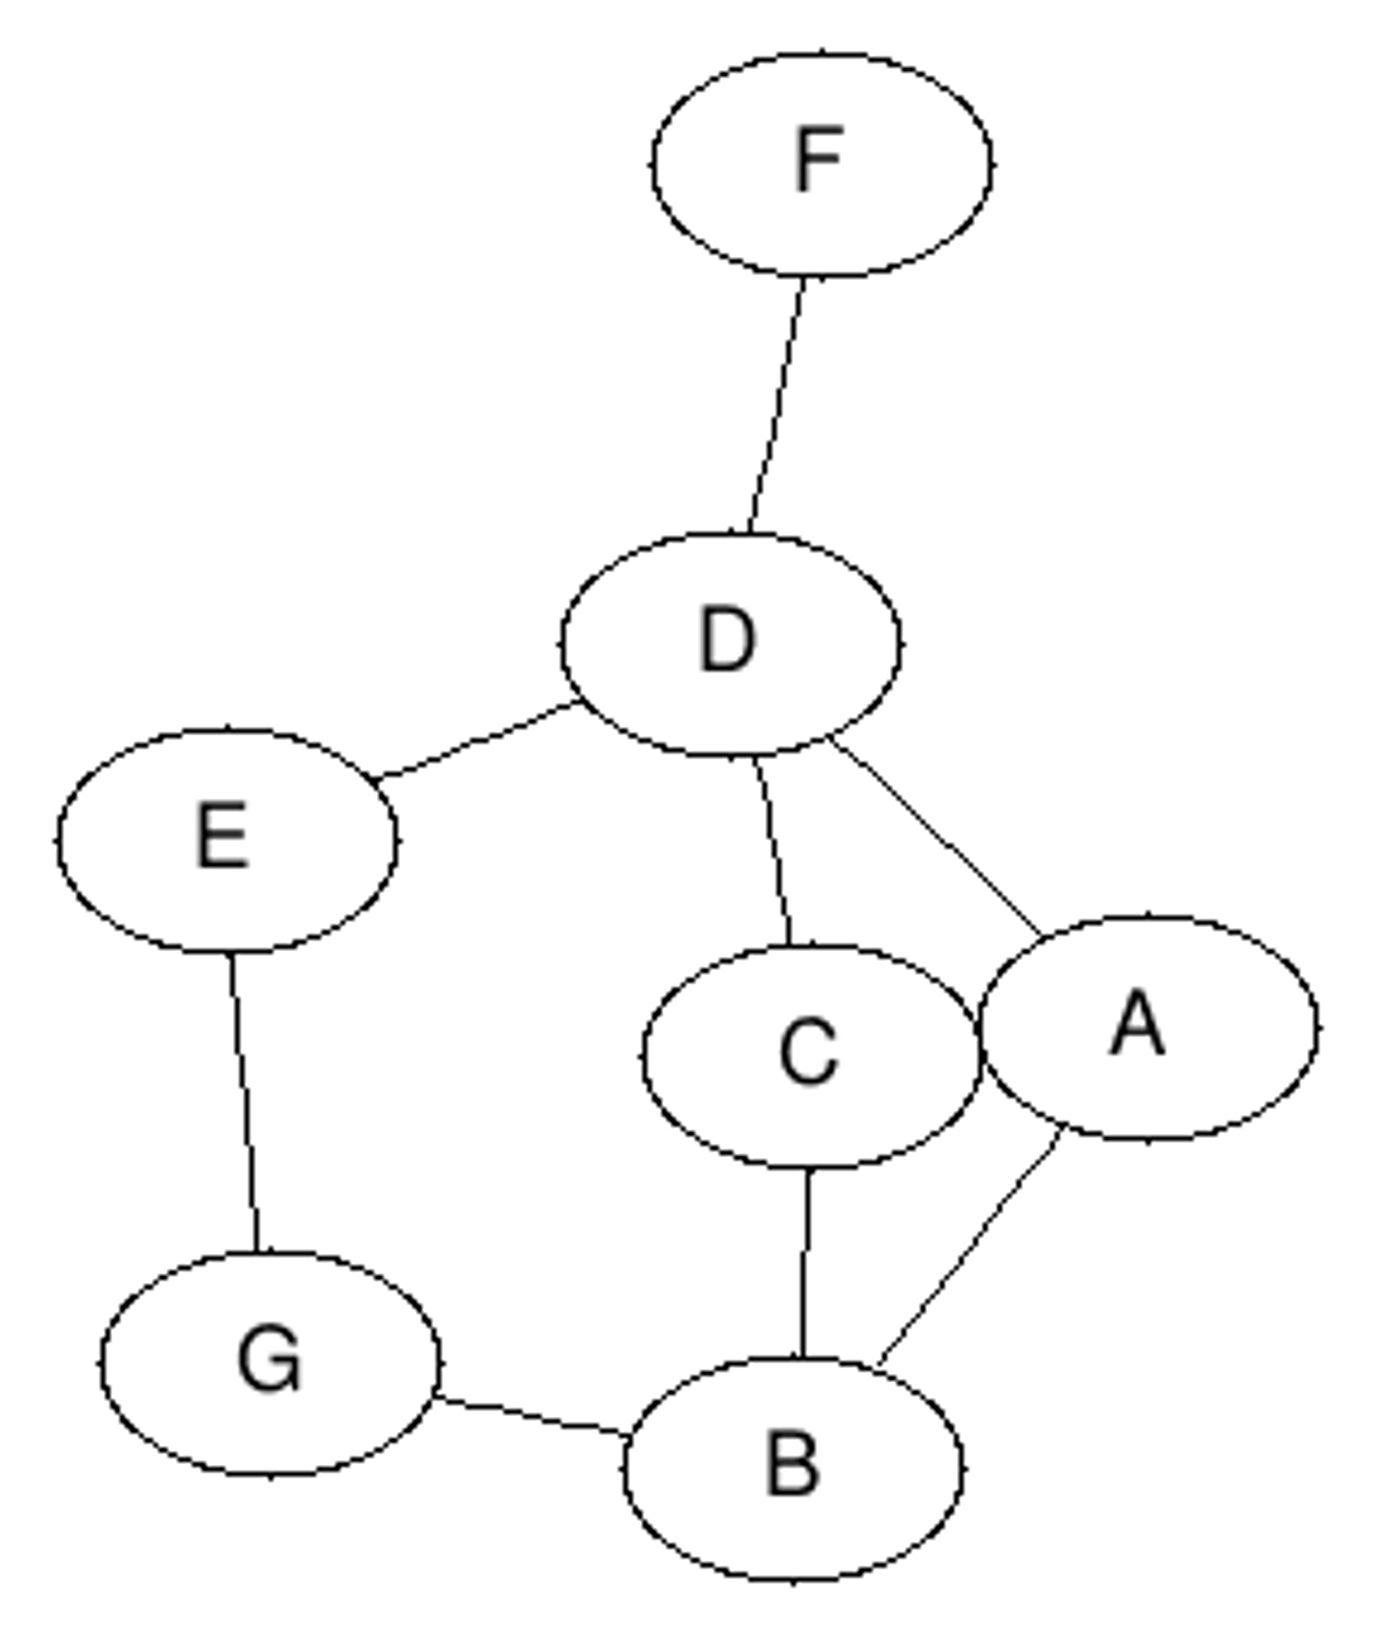
\includegraphics[width=0.6\textwidth]{pictures/neato_example.png} 

	"fdp - \"spring model\" layouts similar to those of neato, but does this by reducing forces rather than working with energy."\cite{graphviz_layout} (fdp - "pružinový model" podobný
	modelu neato, místo práce s energií redukuje síly.) Fdp je další z rozložení pro neorientované grafy, ještě více zmenšuje plochu grafu tentokrát i s ústupkem ohledně překrývání,
	uzlů hranami. Pro grafy které potřebuji vytvořit se jedná o ten nejhorší algoritmus z pěti zde zmíněných. V uzlech jsou zapsány data o zařízeních a hrany překrývající tyto uzly
	působí rušivě. Zároveň není třeba šetřit místem neboť ve výsledné aplikaci je možné přibližovat a popotahovat graf dle libosti uživatele. Fpd tedy není algoritmem vhodným pro tuto
	situaci.
	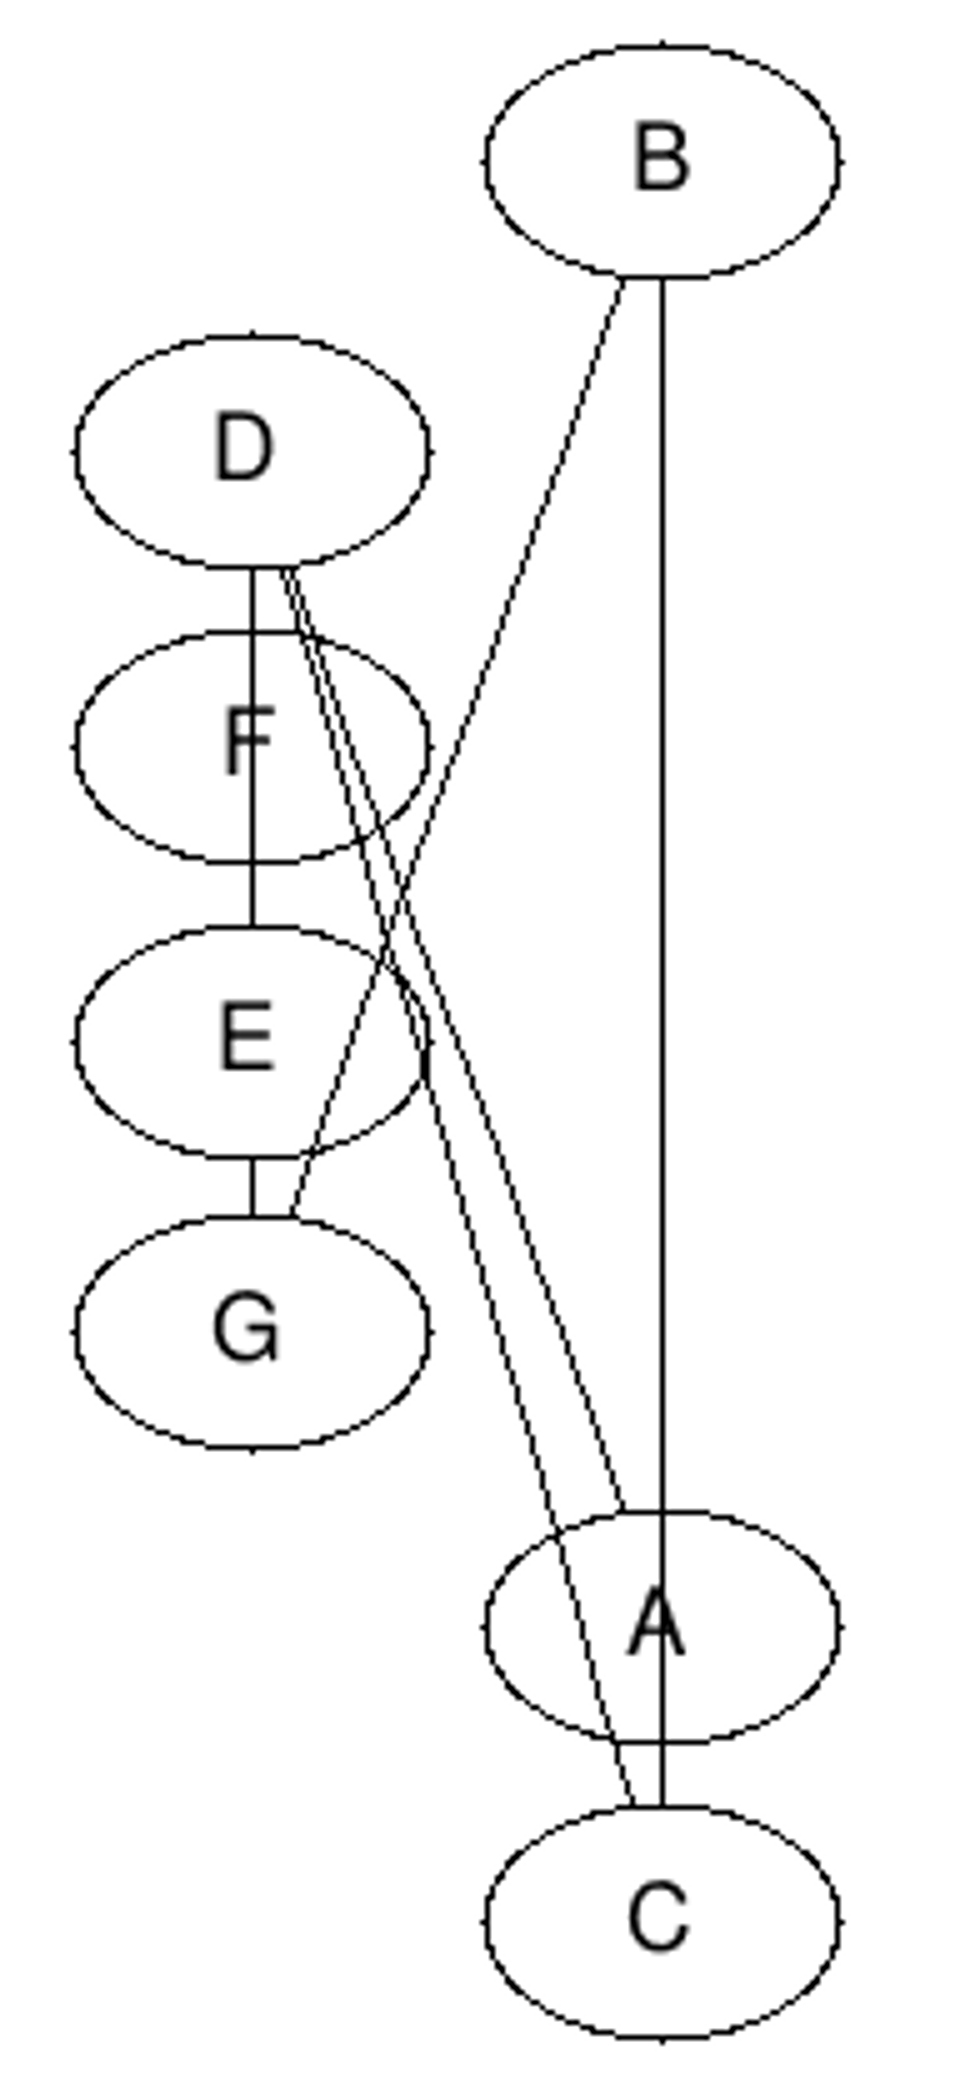
\includegraphics[width=0.6\textwidth]{pictures/fdp_example.png} 

	"twopi - radial layouts\[...\].  Nodes are placed on concentric circles depending their distance from a given root node."\cite{graphviz_layout}(twopi - paprskovité rozložení. Uzly
	jsou umístěny na soustředných kruzích podle vzdálenosti od kořenového.) Použitím paprskového rozložení dochází k strukturalizaci grafu, tím pádem by se algoritmus twopi mohl zdát 
	dobrou volbou pro uskutečnění cíle který jsem si vytyčil. Ovšem přidáním dalších 2 uzlů, které způsobí rozvětvení grafu se strukturalizace začne vyvíjet neakceptovatelným směrem.
	Oba případy jsou vidět na obrázku. Strukturovanost do kruhů by, dle mého názoru, uživatele zbytečně mátla. Je důležité mít kořenový uzel, ovšem jeho umístění doprostřed je špatnou
	volbou.
	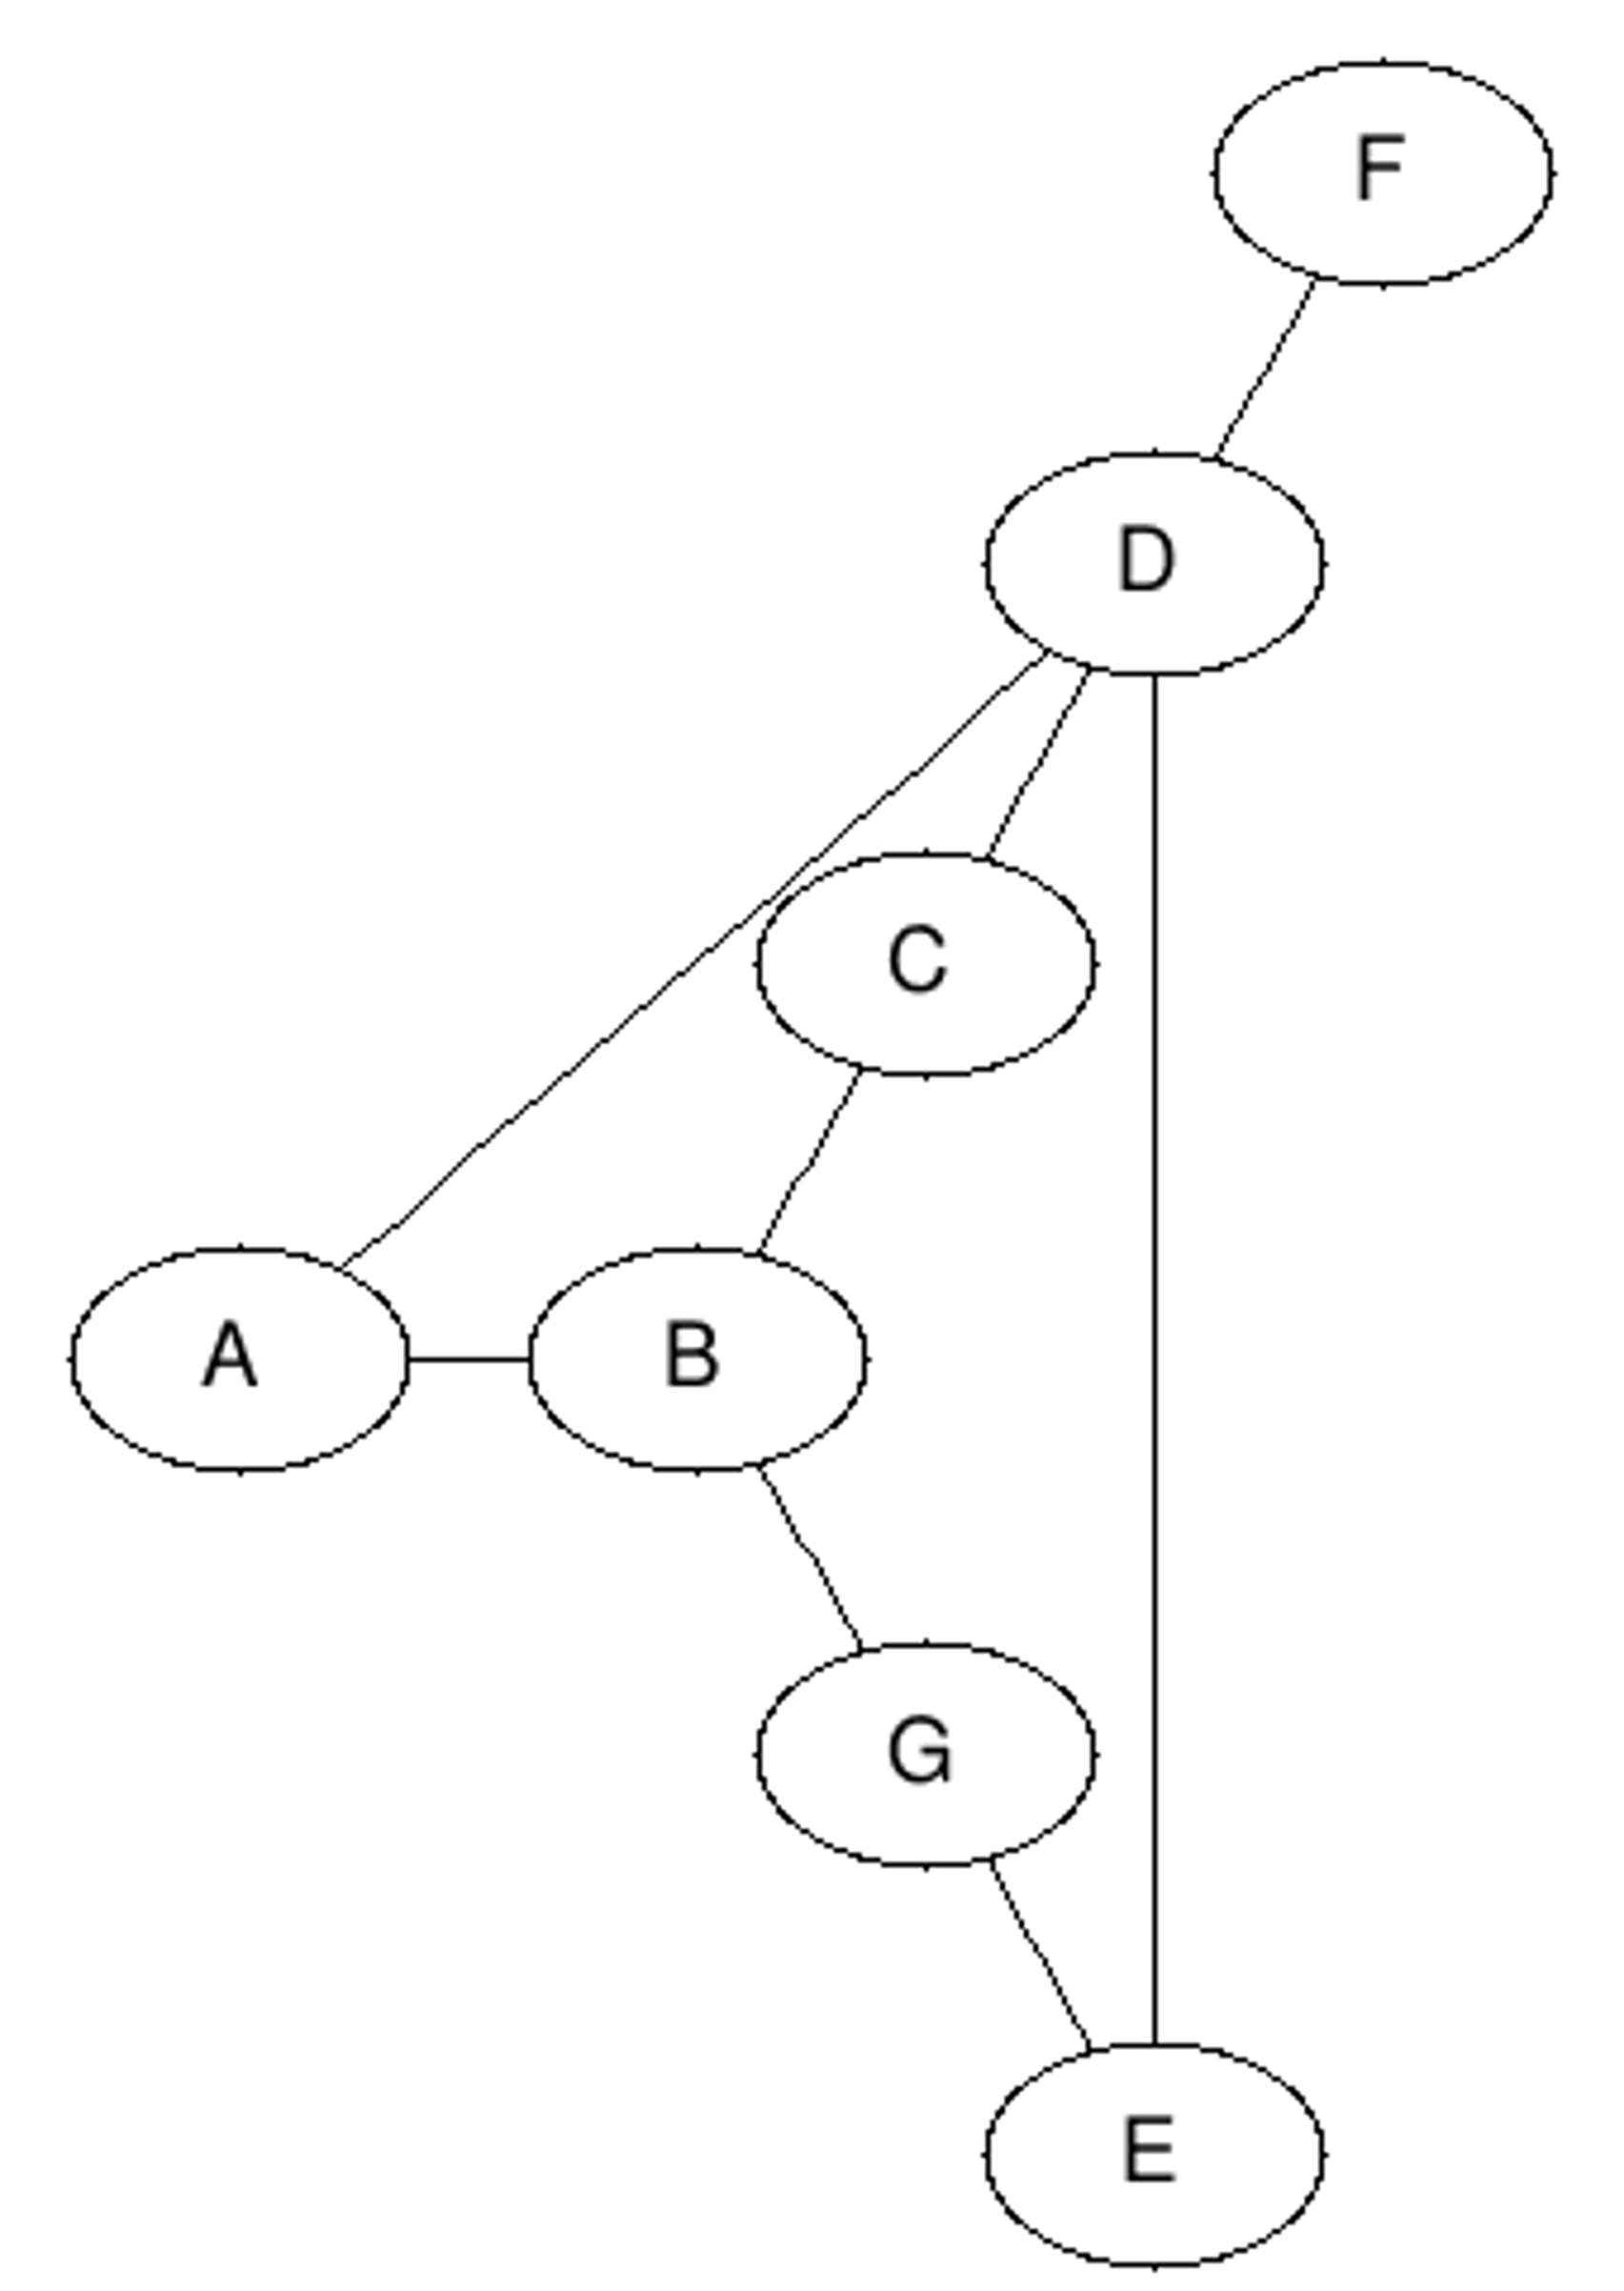
\includegraphics[width=0.6\textwidth]{pictures/twopi_example.png} 
	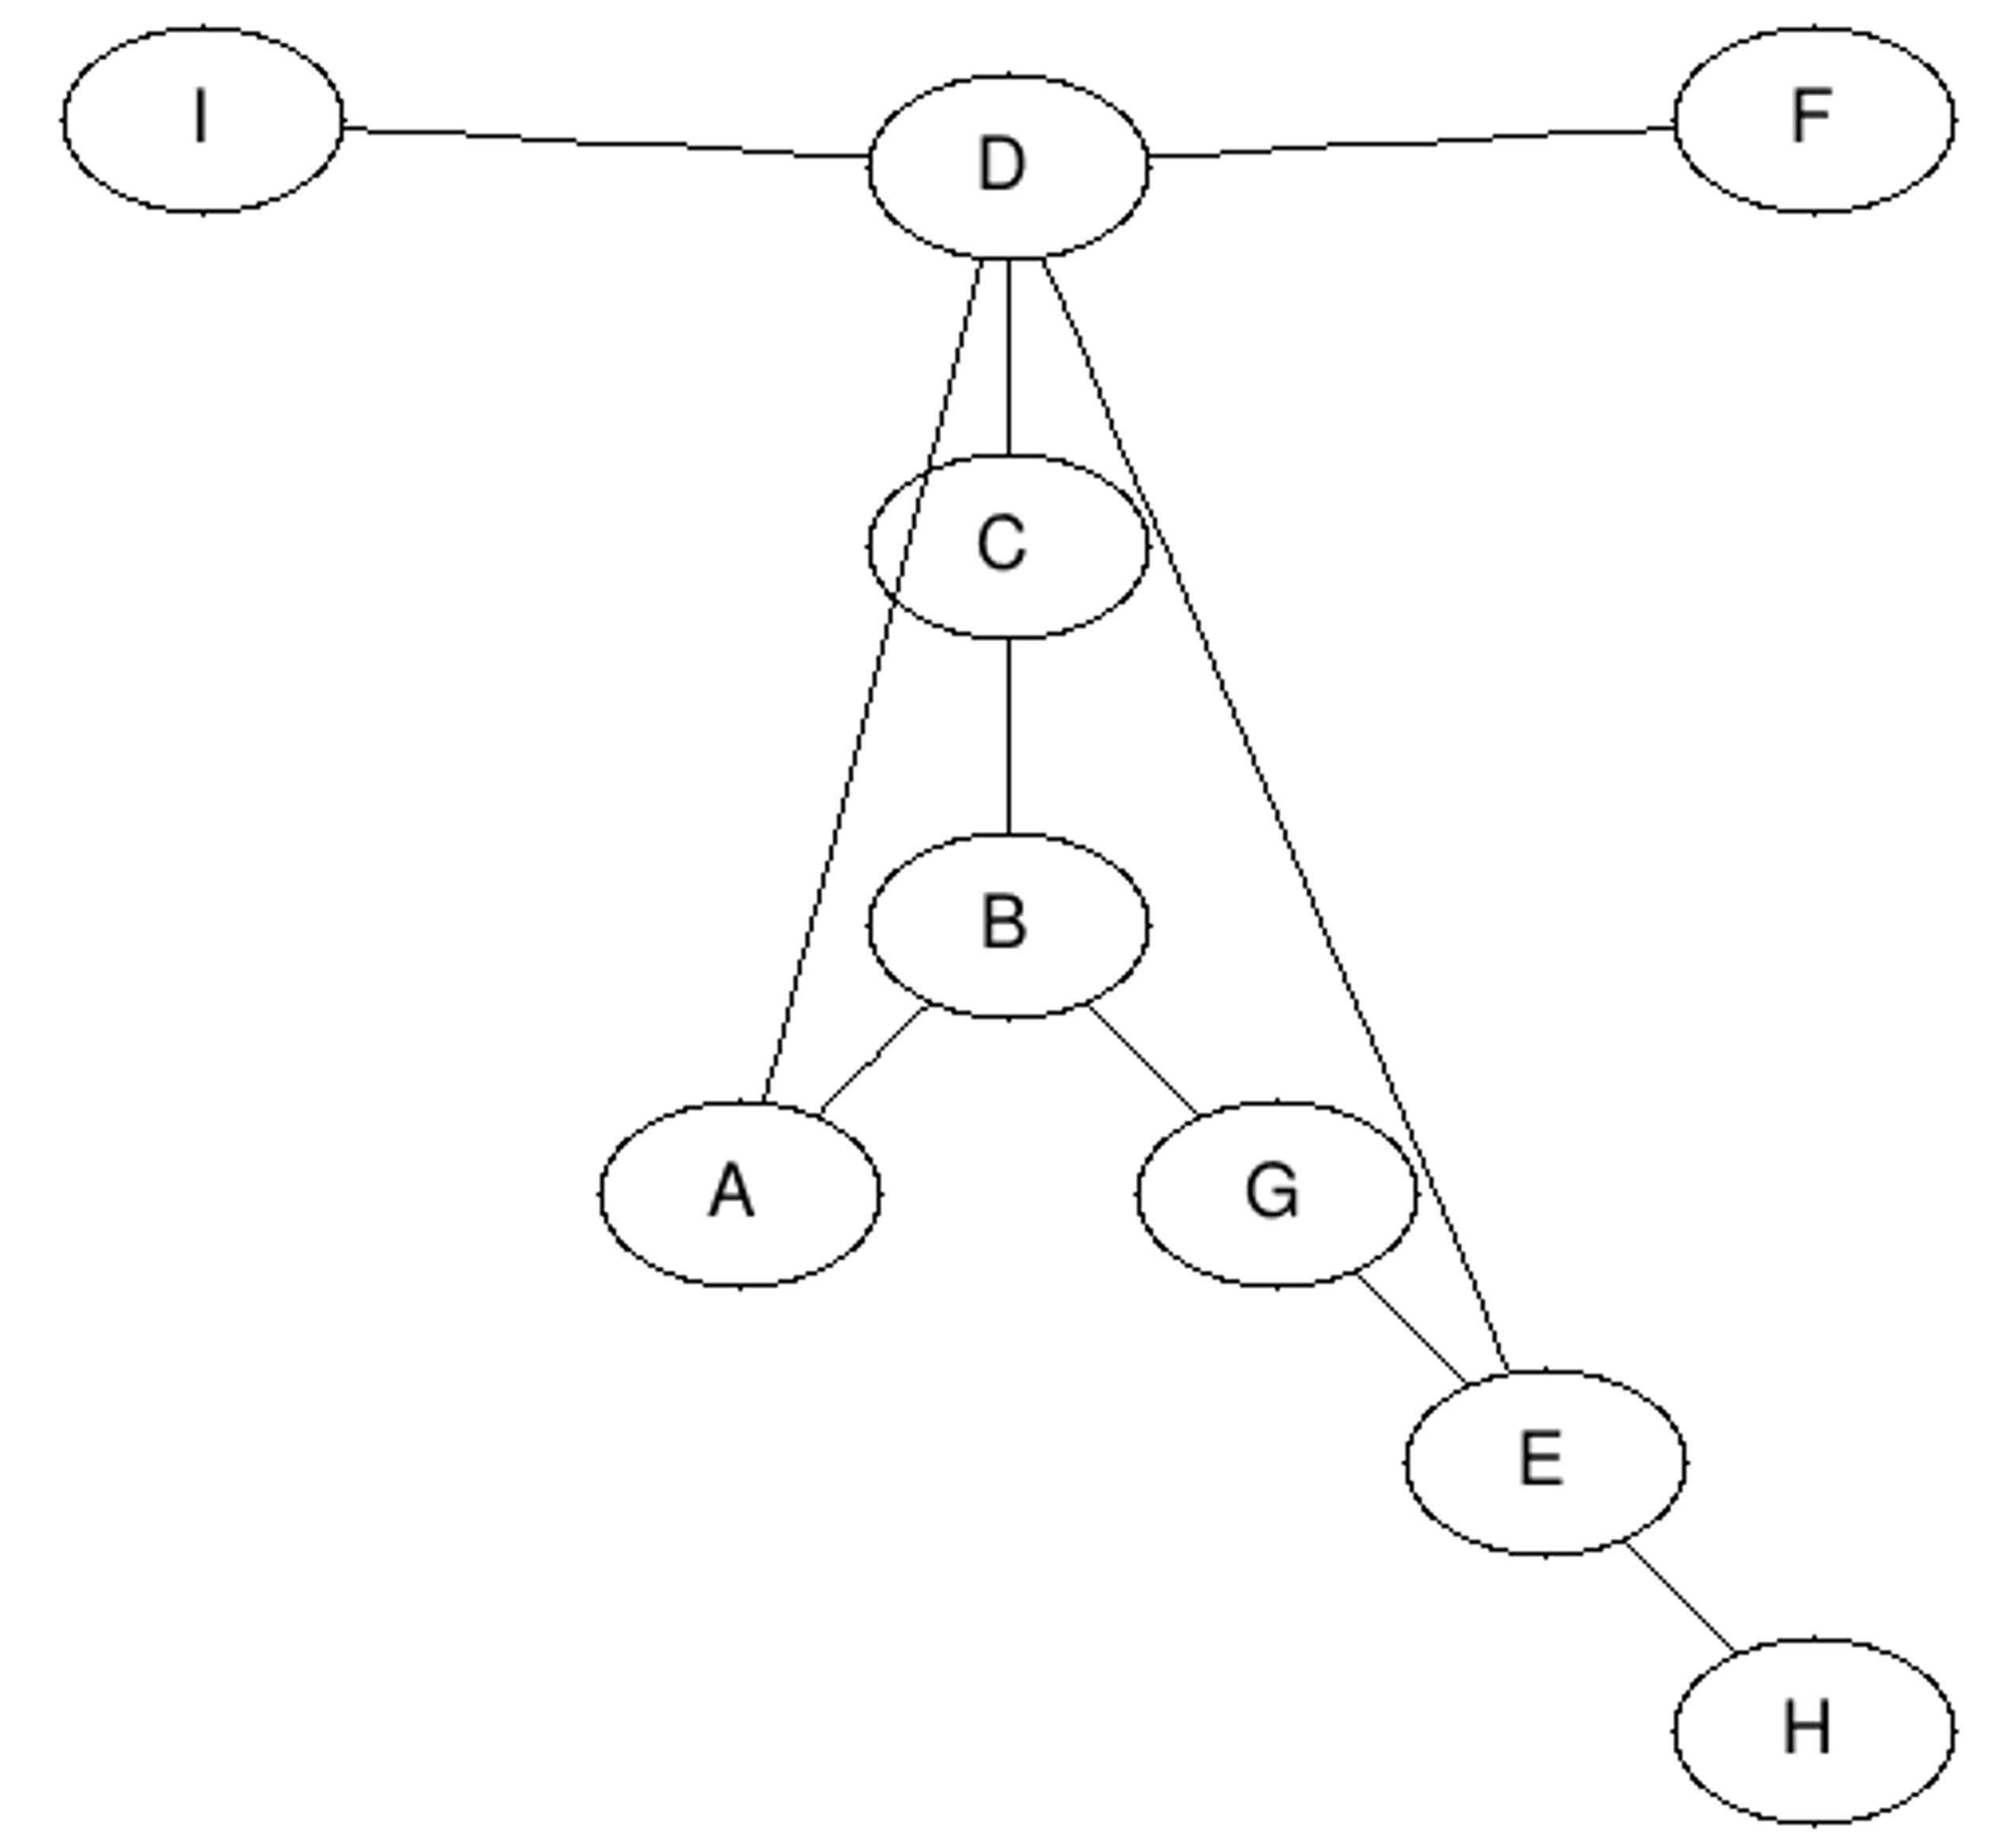
\includegraphics[width=0.6\textwidth]{pictures/twopi_example_2.png} 

	"circo - circular layout \[...\]. This is suitable for certain diagrams of multiple cyclic structures, such as certain telecommunications networks."\cite{graphviz_layout} (circo -
	kruhové rozložení. Je vhodné pro určité diagramy s několika cyklickými strukturami jako jsou telekomunikační sítě.) Jak už je zmíněno v dokumentaci, grafy používající rozložení 
	circo se hodí jen k nemálo specifickým účelům. Jak vidíme na obrázku, opět se setkáváme s nehierarchickým grafem. Algoritmus circo rozhodně má své využití ale není to náš případ. V
	situaci kdy připojujeme úložná zařízení v systému Linux se jen obtížně dostaneme do cyklických odkazů. Samotná podstata připojování úložných jednotek by měla zabraňovat těmto
	situacím. Pokdu bychom už takovou situaci vytvořili jedná se zcela určitě o chybu buď používaných nástrojů nebo chybu uživatelské konfigurace. 
	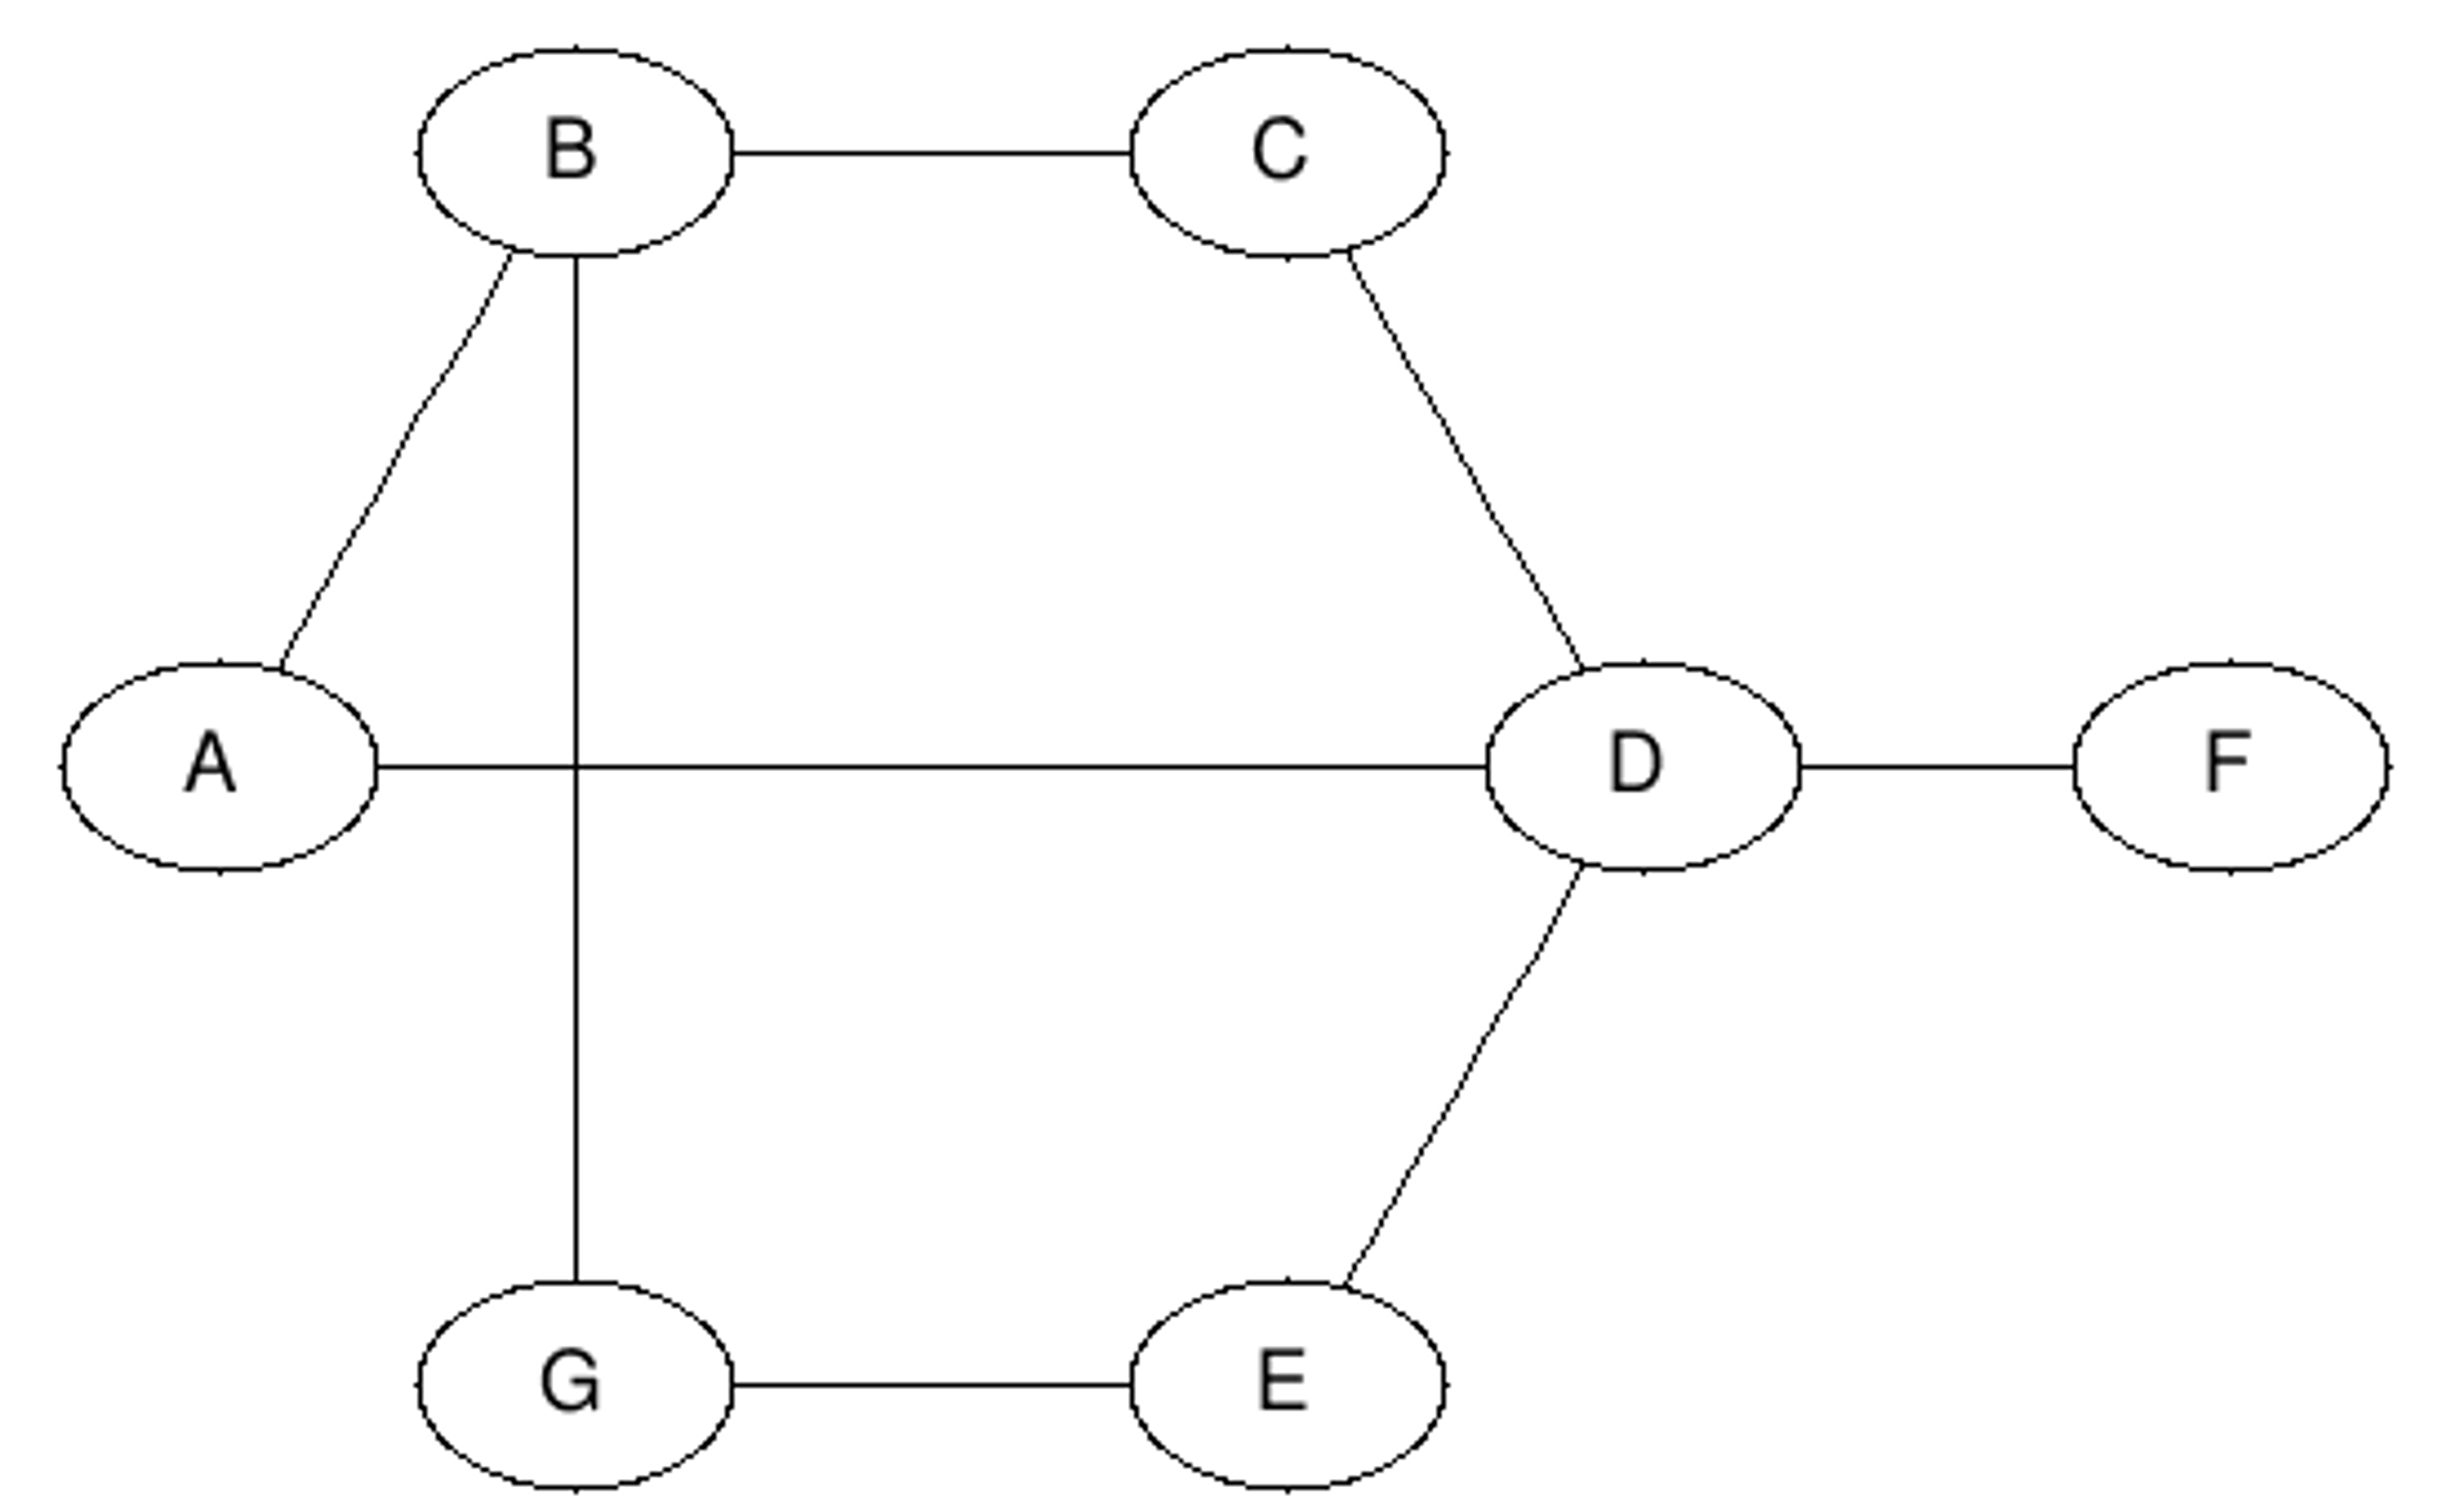
\includegraphics[width=0.6\textwidth]{pictures/circo_example.png} 

	Algoritmem který nakonec zbývá po aplikování vyřazovací metody je algoritmus dot. Po odstranění ostaních možností je jediným co zbývá, bez dalších konkurentů mezi kterými je třeba 
	rozhodovat. Základem pro mé rozhodnutí je stromová struktura. Ostatní typy rozložení nesplňují tuto podmínku, snad až na rozložení twopi. Twopi ale nelze použít kvůli jeho větvení
	ke kterému bude docházet velmi často. Navíc má problémy s dměmi a více kořenovými uzly, nezařazuje je k sobě pokud nejsou spojeny hranou. V prostředí kde je využívána technologie
	RAID jde o zcela nepřijatelnou vlastnost. Je potřebné aby disky logicky náležící k sobě tak také byli vizualizovány. Jen dot splňuje tuto podmínku. Není problém směrovat grafy 
	vytvářené rozložením dot shora dolů či zleva doprava, zmíněné chování jde nakonfigurovat. Tím odpadá poslední argument pro použití twopi které na prvním příkladě graf situuje jako
	jdoucí zleva doprava.

\chapter{Návrh aplikace}
\section{Návrh kódu}
	Aplikace je napsaná v jazyce Python s částečným využitím objektového paradigmatu. Důvody které mě vedli k výběru programovacího jazyka jsou zmíněny v úvodu práce. Objektové 
	paradigma jsem zvolil, protože jsem na něj nejvíce zvyklý. Ač je má aplikace pouze malým dílem bez tříd s dědičností přesto je obsahuje. Z několika důvodů. Za prvé, objekty logicky
	dělí program do částí ve kterých se snadno orientuje a které spolu souvisí. Tak jsou rozděleny i mé třídy. Tj. třída pro načítání dat, pro tvorbu grafu, pro uzly, pro hrany atd.
	Za druhé, objektové programovaní je dnes defacto standartem a velká část nově vznikajících programů je psána s použitím jazyků podporujících objektové programovaní. Za třetí,
	objektové programování usnadňuje spoluprácí a čtení kódu ostatnímy programátory. Jelikož rozšiřuji svobodný software je pravděpodobné že na něm někdo bude v budoucnu pracovat
	a rozšiřovat jej. S použitím objektů bude mít usnadněnou práci.
	
\subsection{Třída Visualization}
	Hlavní třída mého programu je nazvaná Visualization. Obsahuje základní atributy a metody potřebné pro chod aplikace. Můžeme si jí představit jako centrální řídící jednotku. Ostatní
	třídy na ni navazují ať už přímo nebo nepřímo (přes jinou třídu). 

	Konstruktor třídy visualisation vytváří dva seznamy. Seznam uzlů a seznam hran. Víc není potřeba. S oběma seznamy už pracují hlavně funkce v jiných třídách. Nejdůležitější funkcí
	je funkce create_graph. Tato funkce se dá volat z příkazové řádky i z grafického rozhraní. Její argumenty jsou jméno a cestake grafu a výsledkem je svg soubor obsahující graf. 
	V~případě spouštění z grafického rozhraní okamžitě dojde k zobrazení grafu v okně aplikace. V případě spuštění z příkazové řádky jen k jeho uložení v definovaném umístění. 

	Třída obsahuje i pomocnou funkci prepare_nodes, procházející jednotlivě uzly v seznamu uzlů a na každém spouští funkci prepare. Detailně funkci prepare rozeberu u popisu uzlu. Tím
	přemění data z blivetu na data vhodná pro graphviz. Kromě toho jsou utříděna textová data k vypsání po rozkliknutí uzlu uživatelem. Funkci jsem přidal do této třídy proto, že 
	seznam uzlů je její atribut. Třída ve funkci načte data, přetvoří je a pak vypíše. Strukturu tohoto procesu bych chtěl nadálezachovat i například po dalším rozšíření.  

\subsection{Třída pro načítání dat}
	GvInput slouží k načítání dat z blivetu. Jednoduše si blivet naimportuje jako modul, vytvoří si objekt obsahující celou knihovnu. Aktuální nastavení knihovny blivet vyžaduje před 
	každým načítáním dat spustit funkci reset(). Tato funkce projde dostupné úložné kapacity a vytvoří strom zařízení (device_tree). Stejně tak naplní i seznam (struktura list) těmi
	stejnými objekty. Můj program projde tímto seznamem (blivet.devices) a u každého prvku nejdříve zkontroluje zda se nenachází na černé listině. Zde se nachází věci jako jsou 
	výměnná média. Při instalaci jsou zbytečná a jen by na grafu překážela.

	Dalším krokem je vytvoření objektu reprezentujícímu uzel grafu, jeho zpracování a přidání do vlastního seznamu uzlů, fungujícímu jako převodník mezi blivetem a graphvizem. Při
	přidávání do seznamu se uzly zároveň třídí pomocí přepínače a jsou jim nastavovány barvy a tvary. Vše co potřebujeme pro zobrazení uzlu se ukládá ihned při průchodu seznamem. 
	Tím dosáhneme pouze jednoho průchodu. Uzly si už pak informace zpracují sami. V případě že by nebyl uzel rozpoznán, nenastane situace kdy by program zhavaroval. Jednoduše 
	se při vytvoření použije přednastavená barva a tvar (bíla, elipsa).

	Nastavování tvarů a barev je řešeno obdobně jako užití příkazu switch v jazyce C či podobných. Python tento výraz přímo neobsahuje a tak jsem byl nucen použít funkci obsahující 
	sérii if příkazů. Po vyhodnocení jedné z větví na hodnotu pravda se spustí jiná funkce nastavující vzhled uzlu. Konkrétní příklad, k na seznamu je diskový oddíl. Není na blacklistu,
	proto postupuje dál. Konstruktoru třídy Node jsou předány informace z blivet.device. Poté je uzel předán funkci process_node která jej rozpozná jako oddíl a spustí funkci 
	nodeIsPartition. V ní je výsledný uzel obarven světlou barvou a je mu nastaven tvar "box", neboli tvar s ostrými rohy. Poté je uzel přidán do seznamu node_list. Také je na
	standardní výstup vypsána hláška o přidání nového členu seznamu. Uživatel tak má přehled, které uzly jsou přidány. Zařízení je identifikováno svým jménem a typem.

	Po přidání uzlu se přidávají hrany. U každého uzlu program projde seznam jeho rodičů a vytvoří od nich hrany zpět k aktuálně vytvářenému uzlu. Musím postupovat tímto způsobem, neboť
	knihovna blivet nemá jiné propojení mezi zařízeními než seznam rodičů. Stále ale stačí projít seznam zařízení jen jednou. Hrana se vývtáří pomocí koncových uzlů které má spojovat.
	Pokud jeden chybí je vytvořen. Opět nedochází k havárii programu. Pokud už uzel existuje je k němu hrana připojena. Pokud neexistuje je později, až přijde na řadu obarven.

\subsection{Třída Node}
	Třída pro uzly celkem nekomplikovaná, obsahuje převážně funkce pro nastavení vzhledu. Nejdůležitější informace se ukládají už v konstruktoru, opět jako ochrana slouží nastavení
	prázdných řetězců tam kde by vstupní informace chyběly. Kromě konstruktoru obsahuje třída Node také funkce change_color a change_shape nastavující vzhled. K funkci change shape 
	jsem muset vytvořit i pomocnou funkci change_style_safely. Pomáhá vytvořit styl uzlu se zakulacenými rohy. Graphviz řeší tuto situaci přidáním klíčového slova rounded k už 
	existujícímu stylu. Pokud je styl nastavený na obdélník s ostrými rohy ("box") je třeba přidat slovo rounded a obě slova oddělit čárkou. Výsledek musí vypadat takto "box, rounded"
	na pořadí slov nezáleží.

	Ukládání atributů a gv_atributů (atributů pro graphviz) je řešeno pomocí slovníků. Použití slovníků umožňuje libovolně přidávat a ubírat počty atributů. Původní návrh s proměnnými
	pro atributy jsem zavrhl. Atributy rozumíme informace o nastavení úložných zařízení které se později vypisůjí ke každému uzlu. Jedinou výjimku tvoří jméno a typ zařízení neboť jde
	o identifikační atributy a jejich neexistence by znemožnila fungování programu. Rozhodl jsem se oddělit atributy pro knihovnu graphviz do samostatného slovníku. Díky tomu je při
	vykreslování grafu možné jen projít záznamy a vytvořit z párů klíč, hodnota páry atribut ulzu, hodnota v grafu. 

	Poslední pomocnou funkcí nacházející se v tříde Node je fukce prepare. Připravuje textová data pro prezentaci na graf. Projde všechny záznamy ve slovníku attributes a spojí je do 
	jednoho řetězce obsahující znaky nového řádku "\n". Předtím je možné flexibilně měnit počet a data textových informací. Po té co je spuštěna funkce prepare je její výsledný řetězec
	uložen do atributu gv_atributu label, připraven pro použití Graphvizem.

\subsection{Třída Edge}
	Třída pro hrany v sobě neskrývá žádná tajemství. Obsahuje akorát konstruktor a funkce pro získání počátečního a koncového uzlu. Konstruktor bere za své argumenty právě tyto dvě 
	proměnné. Proměnnou node_from, počáteční uzel a proměnnou node_to, koncový uzel. I přesto že neobsahuje moc funkcí jsem se rozhodl vytvořit dedikovanou třídu pro hrany. Z mého 
	pohledu jde o lepší postup než hrany řešit jinde. Takto je pro každý element v grafu dedikovaná třída se kterou lze pracovat.

\subsection{Třída pro vytváření grafů}
	Vytváření grafu samotné také není ničím zvlášť složitým, nicméně pro použití v mé aplikaci je potřeba výsledný graf dále upravit. Rozeberme funkce ve ve třídě output chronologicky,
	tak jak jou použity. Tradičně konstruktor přebírá seznam uzlů a hran. Volá funkci vytvářející graf se jménem createGvGraph a předává jí své argumenty. 

	CreateGvGraph nejprve vytvoří orientovaný graf pomocí graphvizu. Poté projde seznam uzlů a pomocí graphvizu vytvoří každý uzel v nově utvořeném orientovaném grafu. To samé udělá i
	s hranami. Funkce pro vytváření uzlů graphviz.node bere jako první argument jméno uzlu. První argument je povinný, jméno uzlu. Ze stejného důvodu je povinný i argument jména
	při vytváření v seznamu uzlů. Druhý argument ze tří je atribut label. Jde o dlouhý string rozdělený znaky dalších řádků ("\n") jak je vysvětleno výše v částí věnující se třídě Node.
	Poslední argument je seznam zbylých atributů které dokáže graphviz zobrazovat. Je předán jako celý seznam a po jeho rozbalení se aplikují nastavení vzhledu uzlu. Na konci je celý
	graf vrácen návratovou hodnotou.

	Druhá funkce se nazývá createSvg. Jejím úkolem je přepsat graf do formátu svg. Používá knihovní funkci grafu jménem pipe. Pipe dokáže vytvářet i jiné formáty ale ty nejsou v tuto
	chvíli důležité. Svg formát byl vybrán prto že v něm lze aplikovat javascript a tím dosáhnout interaktivity. Konkrétně se jedná o možnost zvětšovat uzly, posouvat a zoomovat graf.
	Tyto funkce jsou implementovány popíšu je později ale postup implementace si popíšeme hned.

	Javascriptový skript vkládá pomocná funkce insert_JS_to_graph, přebírající jeden argument a to řetězec obsahující svg grafu do kterého se má vložit. Zmíněný řetězec je výstupem funkce
	graphviz.graph.pipe s argumentem format="svg". 

	Funkce insert_JS_to_graph nejprve nastaví defaultní jmenný prostor (namespace, funkcionalita XML jazyků schopná rozlišovat různé elementy se stejným názvem) z "ns0" na "" (prázdný 
	řetězec). Svg by bylo validní i se jmenným prostorem "ns0" nicméně standartně po vygenerování knihovnou graphviz tento jmenný prostor není přítomný a považuji za lepší do svg 
	zasahovat co nejméně. 

	Dále se svg nahraje do objektu ElementTree (ET). ET je obsažen v základní knihovně jazyka Python, je jednou ze tříd pro práci s daty ve formátu XML. Vytváří v paměti stromovou
	strukturu stejnou tak jak je reprezentována načteným XML souborem. Obsahuje funkce pro čtení rodičů i potomků, funkce pro vytváření, přidávání a mazání elementů a vyhledávání pomocí 
	XPath. Element Tree lze nahrtá ze soubory či z řetězce. Využívám funkci načítání z řetězce. Poté vyberu kořenový element a upravím jeho atributy.

	Úprovou atributů se rozumí přidání odkazu na "xmlns:xlink", kvůli možnosti odkazovat na soubory s Javascriptem. Také je třeba odstranit atribut viewBox aby mohlo fungovat posouvání
	grafu. Zároveň je třeba připravit atribut "viewport" u prvního potomka elementu svg. První potomej je kořenový uzel zobrazovaného grafu, vždy nese id "graph0". Pomocí XPath výrazu jej
	najdu a přiřadím mu zmíněný atribut.

	Poté už stačí jen vytvořit nový element s cestou k Javascriptovému souboru a tento element přidat jako prvního potomka kořenového elementu svg. Funkce insert_JS_to_graph vrací celý
	Element Tree.

	Po návratu z funkce insert_JS_to_graph použijeme metodu write k zapsání svg do souboru kde je připraveno k zobrazení.

\subsection{Třida Gui}
	Můj program lze používat jak dávkově z příkazové řádky tak interaktivně s pomocí grafického uživatelského prostředí. Dávkový režim nabízí pouze možnost vygenerovat graf v určitém 
	umístění. Interaktivní režim nabízí možnost graf ihned prohlížet. Variací na interaktivní režim je také okno s grafem které se zobrazuje při instalaci jako vezualizace změn prováděných
	instalárorem. 

	Třída gui obsahuje vše potřebné pro obsluhu uživatelského rozhraní. Je naprogramována s pomocí nejrozšířenější linuxové knohovny pro uživatelská rozhraní Gnome toolkit (GTK). Jde o 
	obyčejné okno s pár tlačítky. Jsou v ní obsaženy ovládací prvky potřebné pro nastavení umístění uložení grafu, tlačítko pro vyvolání kontextové
	nápovědy. A plocha zobrazující samotný graf. Tato plocha je zabrána oknem technologie WebKit. Okno WebKitu je možné vložit do GTK aplikace a tím dosáhnout stejné základní funkcionality
	jakou májí dnešní moderní prohlížeče. V mém případě jde o schopnost zobrazit svg kód a schopnost spouštět Javascript.

	Rizikem které je nutné přijmout jsou možné známe zranitelnosti prohlížečů a nutnost ukládat soubor svg na disku. WebKit totiž zobrazuje svg s pomocí protokolu "file://". Počítač se
	tak ptá sám sebe na existenci souboru v určité cestě definované uživatelem a pokud jej najde zobrazí jej uživateli. Pokud by se k systému dostal útočník mohl by soubor upravit a 
	zanechat v něm škodlivý kód. Nicméně bezpečnost systému není věcí této práce a vychází se z předpokladu, že systém na kterém je vizualizace spouštěna je buď fe fázi instalace nebo
	je již zabezpečen.
	má prohlížeč.

	WebKit je de facto prohlížeč, který je možné vložit do GTK aplikace.

\chapter{Návrh vzhledu}
TBD

\chapter{Ukázky aplikace}
TBD

\chapter{Další možnosti rozšiřování}
	Zadání mé práce je schváleno jako dostatečné pro bakalářskou práci. Přesto jsem během vypracování diskutoval další možné nadstavby a pokračování v práci. Nyní je stručně představím.

	První rozšíření by byla možnost vytvářet XML soubory obsahující informace z grafů. Již existuje aplikace schopná vytvářet XML soubory z blivetu a zase je zpět nahrávat. Její zamýšlené
	použití je vytváření záchytných bodů ke kterým je možné se vrátit v případě havárie instalátoru, přerušení dodávky elektrického proudu či jiné fatální chyby systému. Ideou pro export
	XML z grafu je možnost na systém dostat přesně tu konfiguraci která mi je prezentována.

	Druhým a ambicióznějším rozšířením je schopnost grafu fungovat jako samostatný konfigurační nástroj. Graf by nejenom zobrazoval data která mu byla poskytnuta ale také je byl
	schopen upravovat a předávat nová data zpět aplikaci blivet, popřípadě instalátoru. Například by bylo možné přesouvat logické oddíly LVM mezi různými skupinami svazků jednoduchým 
	přetažením myší stejně jako dnes kopírujeme soubory přetažením jejich ikony. Nové oddíly by byly vytvářeny také přetažením z nějaké nabídky předpřipravených uzlů. Konkrétní velikosti
	a jména zařízení by se editovaly s pomocí textových polí v každém uzlu.
	
	Největším problémem který by bylo třeba vyřešit je načítání svg a informací z něj zpět zároveň s ukládáním informací z prohlížeče. 
	Jedním z možných postupů by byla úprava XML načítače tak aby fungoval i pro svg graf aktuálně zobrazovaný uživateli. Uživatel by přetvořil graf podle svých představ, poté spustil 
	konfiguraci a ta by přenesla stav do blivetu a provedla změny v úložném prostoru systému. 

	\printbibliography

\end{document}
